\documentclass{report} % Add the document class
\usepackage{graphicx} % For including graphics like logos
\usepackage{lipsum}   % For dummy text
\usepackage{setspace} % For line spacing
\usepackage{fancyhdr} % For custom headers and footers
\usepackage{geometry} % For page margins
\usepackage{amsmath} % For mathematical equations
\usepackage{enumitem} % For customized lists
\usepackage{amsfonts} % For the \forall symbol
\usepackage{multicol} % For multiple columns if needed
\usepackage{enumitem} % For customizing lists
\usepackage{hyperref} % For hyperlinks for table of contents
\usepackage{acronym} % For defining acronyms
\usepackage{tocbibind} % For adding list of figures, tables to table of contents
\usepackage{tabularx} % For tables
\usepackage{float} % For tables
\usepackage{longtable}%to split tables over multiple pages
\usepackage{array}
\usepackage{booktabs}

\usepackage{fancyheadings}
%
\pagestyle{fancy}
\fancyhead[R]{
    
\includegraphics[width=0.1\textwidth]{./ReportImages/thws_logo.png} % Adjust path and filename
}
\fancyhead[C]{} 
\fancyhead[L]{} 
\addtolength{\headwidth}{\marginparsep}
\addtolength{\headwidth}{\marginparwidth}

\geometry{top=1in, bottom=1in, left=1in, right=1in} % Set page margins

% Configure the hyperref package to remove red boxes and customize link colors
\hypersetup{
    colorlinks=true,      % Set to true to enable colored links
    linkcolor=black,       % Color for internal links (sections, pages, etc.)
    citecolor=black,       % Color for citation links
    filecolor=black,       % Color for file links
    urlcolor=black         % Color for URL links
}


\begin{document}

% Title Page
\begin{titlepage}
    \centering
    \vspace*{1cm}
    
    \Large \textbf{Technical University of Applied Sciences Würzburg-Schweinfurt (THWS)}\\
    \vspace{0.5cm}
    \Large Faculty of Computer Science and Business Information Systems\\
    \vspace{1cm}
    
    \huge \textbf{Master Thesis}\\
    \vspace{1.5cm}
    
    \Huge \textbf{Electric Motor Modelling via Graph Neural Networks}\\
    \vspace{2cm}
    
    \large \textbf{Submitted to the Technical University of Applied Sciences Würzburg-Schweinfurt in the Faculty of Computer Science and Business Information Systems to
    complete a course of studies in Master of Artificial Intelligence}
    
    \vspace{1cm}
    
    \huge Lilly Abraham\\
    \huge K64889\\
    \vspace{1cm}
    \large To be Submitted on: 11.12.2024\\ % replace with Submitted on
    
    \vfill
    
    \large
    Initial examiner: Prof. Dr. Magda Gregorova\\
    Secondary examiner: Prof. Gracia Herranz Mercedes\\

\end{titlepage}

\newpage % Start a new page


% Including an image on this page
\begin{figure}[h]
    
\includegraphics[width=0.8\textwidth]{./ReportImages/qrcode.png} % Adjust path and filename
    \label{fig:your-image}
\end{figure}

\newpage % Start a new page

\chapter*{Abstract}
\addcontentsline{toc}{chapter}{Abstract}

The thesis explores an approach to predict Key Performance Indicators(KPI)s of topology invariant Interior Permanent Magnet Synchronous Magnets(IPSM) Electric Motors by transforming its geometric, physical and simulation parameters into a graph representation. \\
The KPIs to be predicted are plots on Efficiency grid(3D) and Torque curve(2D).\\
We aim to first parameterize the EM design such that it is feasible to convert into a graph representation. \\
Next, we would create a Graph with relevant attributes and design a Graph Neural Network(GNN)with the graph as input and the plots in the format of vectors as target values.\\
Additionally we may also need to customize the loss function in a way that would smoothen out the plot curves of the prediction values.\\
Then, we would evaluate the predictions with the test target values by experimenting with various hyperparameter tuning settings and as a baseline with an Multi Layer Perceptron(MLP) model of the parameters in tabular form.\\
Finally we will enable the KPI's plot visualisation in a manner presentable to the client Valeo(Automaker Company).\\
Not necessary remove i suppose....
The aim of the Master Thesis is to train a neural network to learn the parameters of Electric Motors and thus be able to predict its KPIs.
The KPIs are 2D and 3D plots on Torque(Mgrenz) curve(Mgrenz) and Efficiency grid(ETA). Other KPIs can be calculated from these two KPIs.
For instance the Vibration Costs are inversely proportional to the Efficieny values predicted. 


\newpage 

\newpage 

\chapter*{Acknowledgement}
\addcontentsline{toc}{chapter}{Acknowledgement}
I would like to thank my supervisor Prof. Dr. Magda Gregorova for her guidance and support throughout the course of this thesis.
Her dedication and commitment to our work has been inspiring for me to the extend that I might have developed a new love for academia. \\
I would also like to express my sincere gratitude to Valeo for providing us with the dataset.
Special thanks are in order to Daniel and Leo for sharing valuable insights of the data from an electromechanical standpoint and for giving me a detailed understanding of my task. \\
I deeply owe my Mother and my Siblings who have been very instrumental in making it possible for me to pursue a Master's degree outside my home country and for the endless support thoughout.\\
Finally, I humble myself before God Almighty for all his blessings and for giving me the strength to persevere and bring my dreams to fruition.\\

\newpage

\newpage

\begin{spacing}{1.2}
    \tableofcontents
\end{spacing}

\newpage

\newpage

\chapter*{Abbreviations}
\addcontentsline{toc}{chapter}{Abbreviations}
\begin{acronym}[TDMA]
  
    \acro{GNN}{Graph Neural Network}
    \acro{MLP}{Multi Linear Perceptron}
    \acro{KPI}{Key Performance Indicator}
    \acro{EM}{Electric Motor}
    \acro{FEM}{Finite Element Method}
    \acro{CNN}{Convolution Neural Network}
    \acro{2D}{2 Dimension}
    \acro{3D}{3 Dimension}
    \acro{Wandb}{Weights \& Biases}
    \acro{MSE}{Mean Squared Error}

\end{acronym}


\newpage

\newpage

\chapter{Introduction} 
In the design of electric motors, vast amounts of data are generated to determine which design of an \ac{EM} fits best to \ac{KPI}s. \\
\ac{KPI}s of an Electric Motor are essential to judge the performance of the motor before it is manufactured. \\
Traditionally these \ac{KPI}s are inferred from a description of an \ac{EM} design via a \ac{FEM} approximating the solutions of the Maxwell’s equations. \\
This process, though well established in the \ac{EM} design, is very time consuming and does not allow for high-throughput engine design optimization. \\
The actual engine data of Valeo is used here as the dataset comprising of multiple variant designs of the Double-V topology.\\
The 3 motor topologies manufactured by Valeo are as below:

\begin{figure}[H]
    \centering
    \begin{minipage}[b]{0.325\textwidth}
        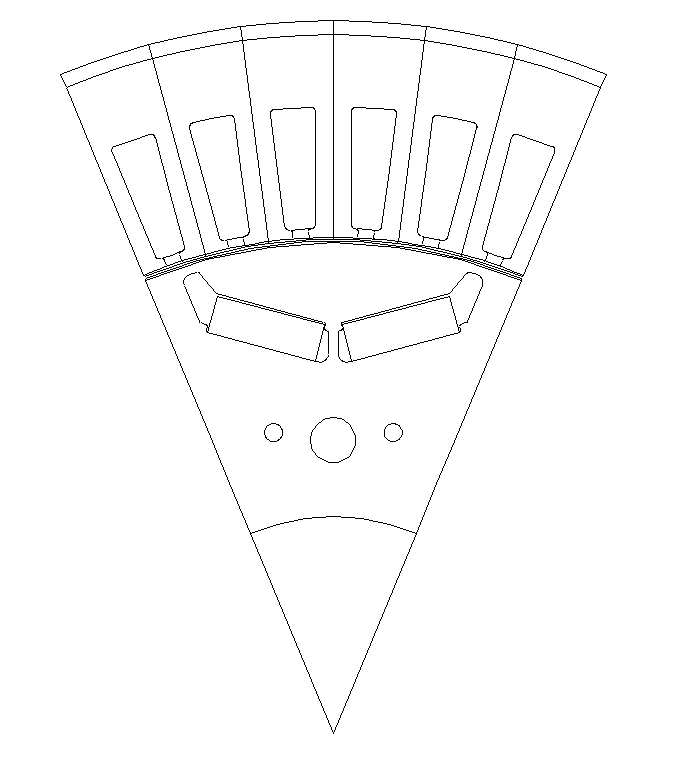
\includegraphics[width=\textwidth]{./ReportImages/1V_Magnet.png}
        \caption{V1 Magnet \\ (Source:Valeo)}
        \label{fig:V1 Magnet}
    \end{minipage}
    \hfill
    \begin{minipage}[b]{0.325\textwidth}
        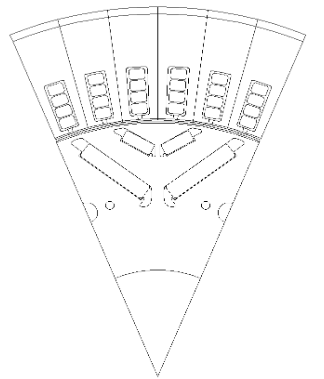
\includegraphics[width=\textwidth]{./ReportImages/2V_Magnet.png}
        \caption{V2 Magnet\\ (Source:Valeo)}
        \label{fig:V2 Magnet}
    \end{minipage}
    \hfill
    \begin{minipage}[b]{0.325\textwidth}
        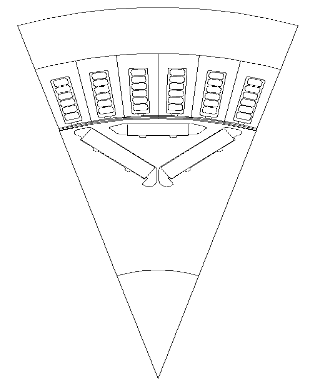
\includegraphics[width=\textwidth]{./ReportImages/Nabla_Magnet.png}
        \caption{Nabla Magnet\\ (Source:Valeo)}
        \label{fig:Nabla Magnet}
    \end{minipage}
\end{figure}
The current approach to predict the \ac{KPI}s of different \ac{EM} design variants is to create a design mesh from the paramteric description of the motor with Matlab.
Multiple FEM simulations is done on this mesh which is then post processed and the intermediary outputs are forwarded to the Motor Builder.
Several Motor builder settings are then adjusted to get the plots of the desired \ac{KPI}s.\\
This master thesis explores a way to do surrogate modelling of the current process as is highlighted in Figure \ref{fig:EM Design Flowchart} by making use of \ac{GNN} or \ac{MLP} for the modelling of electrical engine designs described parameterically. \\
\begin{figure}[H]
    \centering
    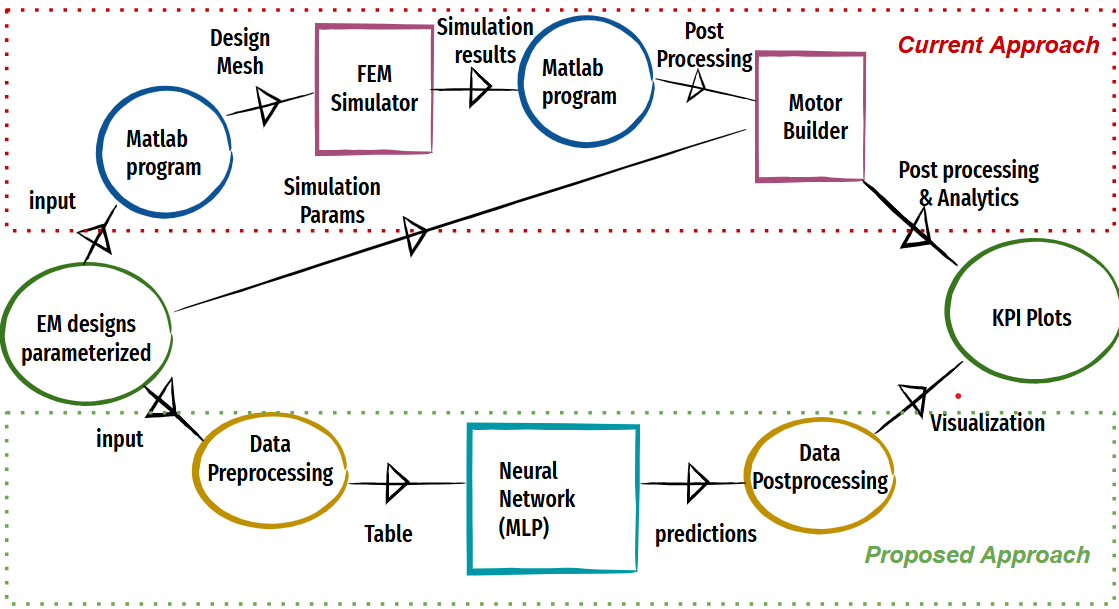
\includegraphics[width=1\textwidth]{./ReportImages/EM_design_flowchart_v2.png} 
    \caption{EM Design Flowchart}
    \label{fig:EM Design Flowchart}
\end{figure}


\section{Objective}\label{sec:Objective}
Our task is to predict 2 KPIs namely the Torque curve and the ETA grid from the parameteric description of topology invariant Electris Motors. \\
The Torque curve is a 2D plot ie, a vector across speed ranges and the ETA grid is a 3D plot ie, a matrix of dimensions torque ranges and its speed ranges. \\
The ETA grid is dependent on the shape of the torque curve and lies within the boundary of the torque curve.\\

\section{Problem Statement}\label{sec:Problem Statement}

Although our training dataset was highly imbalanced to consists majorly of 1 topology ie, Double V Magnet Topology, we aim to build a system that caters to every topology. \\
With the tabular representation of the data, we assign distinct columns to include features from each topology.

Given ETA is dependent on Torque curve, we need to build a model that can predict both these KPIs.\\
However, due to the challenge of predicting ETA grid of varying dimensions for each motor variant, we decided against building a model architecture wherein 2D KPI is dependent on the 2D KPI. \\
This in a way could be overcome if we build 2 models one for the 2D and 3D KPIs and thus feed in the corresponding 2D predictions when training the latter. \\
However, it would be computationally expensive and does not help in the scenario when we might need to generate \ac{EM} parameteric descriptions.
Additionally we deemed it unnecessary as the dimensions of the ETA grid vary with the torque curve and not necessarily the ETA values. \\

Furthermore, we presume graph representation of the data will be more logical than tabular representation due to its ability to grasp the connections within the \ac{EM} structural properties better.
This would be even more realistic with achieving topology invariance than the tabular representation and conserve memory and compute in the long run.
However, we realize that our problem cannot be solved using Homogeneous \ac{GNN} which is relatively simpler and is built on a single node and edge type.
In order to model our problem as a graph, we need to represent it as a Heterogeneous graph. \\

\section{Research Question}\label{sec:Research Question}
\ac{GNN} in general have not been to less explored even so more the heterogeneous \ac{GNN}.
Particularly in the scenario of Electric Motor Modelling, there has been no publications with \ac{GNN}s.
Hence the need to check its feasibility and its performance with our benchmarks on tabular data.
Additionally, Existing Heterogeneous \ac{GNN}s words e.g on social networks involves one large graph with multiple node and edge types. 
However, our problem involves creation of multiple heterogeneous graphs ie, 1 per \ac{EM} variant.\\
Therefore, the applicability of Heterogeneous \ac{GNN}s for our problem is to be seen.\\

\section{Thesis Structure}\label{sec:Thesis Structure}

The thesis is structured to follow sections namely Literature Review, Dataset, Modelling, Experiments and Results, Conclusion, Appendix and Bibliography.\\
In Literature Review section will introduce the works that has already been carried out in this domain. \\
In the Dataset section a detailed insight to how our data is structured is elaborated.\\
In the Modelling section, we introduce the methodologies used to tackle the problem. \\
The Experiments and Results chapter gives an outlook on the outcomes of our work in addition to other findings we unearth.\\ 
Conclusion chapter summarizes the thesis briefly and would also give a small glimpse into areas of improvement. \\
Finally the Bibliography section lists out the articles cited for this thesis.\\
\newpage 

\chapter{Literature Review} 
There has been extensive research in modeling the Electric Motor with \ac{CNN} based on the images of the motor cross-section. \\
However our approach is progressive in the sense that once the \ac{KPI}s are predicted we would like to be able to generate the inputs.\\
Reproducing images is not known to apt given the infamous known fact that AI generated images are faulty instead by generating the parameters of the motor we can be rest assured of more precise results. \\
Hence the need to focus on the inputs as they are with their parametric description.\\
Existing literature also covers works on modelling this work as tabular data using \ac{MLP}s. 
Although this is fairly good forseeing the impact of generating the inverse process yet \ac{MLP}s cannot necessarily learn all the intricacies within motor components. \\
Hence the need to better represent the data typically in the form of graphs and model Graph Neural Networks to achieve the desired results. \\
There has been close to no work of \ac{GNN}s in this domain. However we see progress of \ac{GNN}s in molecular chemistry and social networks usecases from which we draw inspiration.\\

\newpage 

\chapter{Dataset} 
Valeo an automotive company has supplied the dataset consisting of close to 1500 Double V Electric Motor parameters. 
There are close to 196 parameters which comprises of the geometric, physical and simulation properties of the motor.

The geometry of a whole Double V motor is as below

\begin{figure}[H]
    \centering
    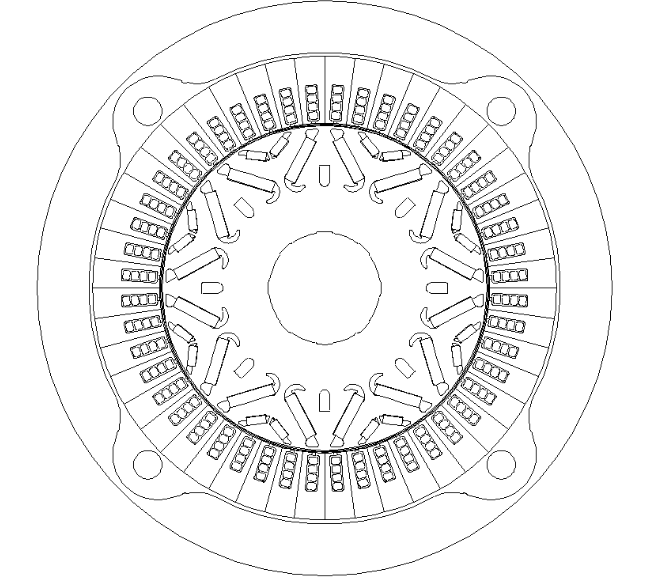
\includegraphics[width=0.5\textwidth]{./ReportImages/FullMotorv2.png} 
    \caption{Complete EM Geometry(Source:Valeo)}
    \label{fig:Full Motor}
\end{figure}

Below is the geometry of 1/8 cross-section of the same motor.

\begin{figure}[H]
    \centering
    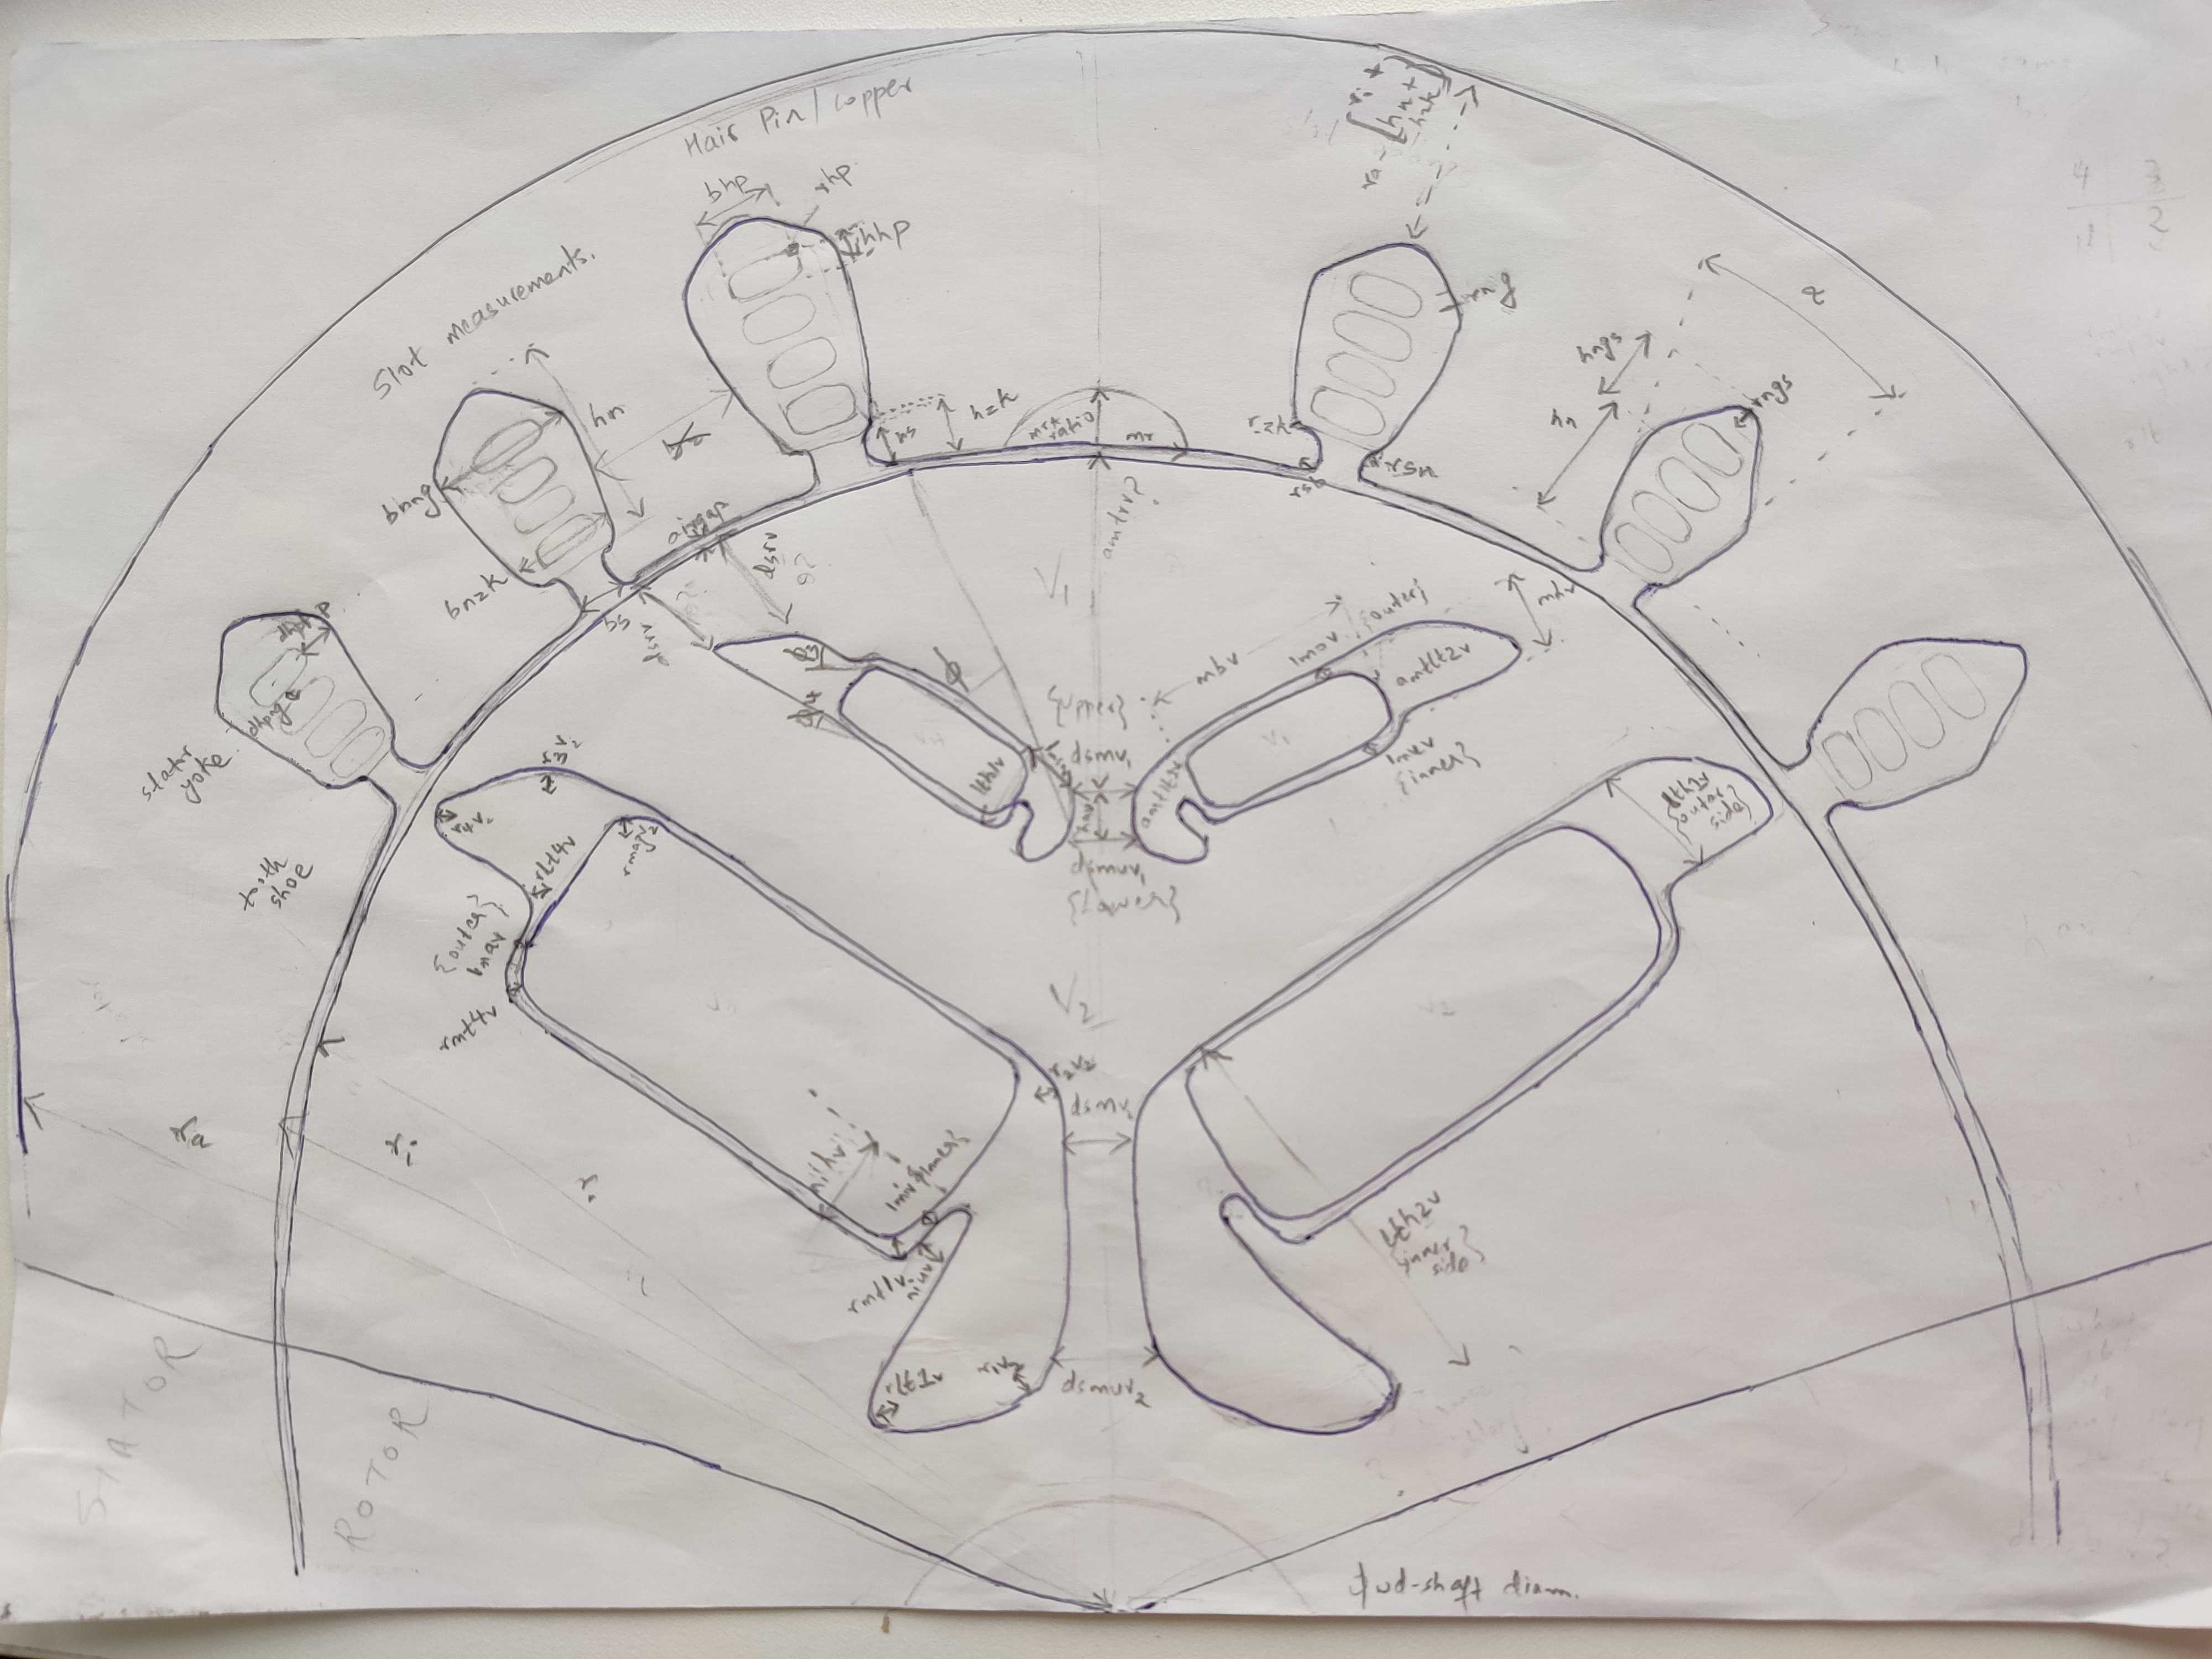
\includegraphics[width=1\textwidth]{./ReportImages/EMCrosssection.jpg} 
    \caption{1/8 Motor Crossection}
    \label{fig:1/8 Motor Crossection}
\end{figure}

\newpage 

Valeo has shared approximately 1500 Excel Workbook files for each motor variant. Each of the excel files contain multiple sheets.
The sheets of interest to us are as below :
\begin{table}[H]
    \centering
    \begin{tabular}{|p{2cm}|p{2cm}|p{11cm}|}
    \hline {\bf Sheet} & {\bf Sheet Name} & {\bf Description}\\
    \hline Motor Parameters & input\_data & 
    \begin{itemize}
        \item Contains the input parameters for the motor model.
        \item Includes geometric, physical, and simulation properties.
        \item Unit dimensions if applicable are generally mm or degrees 
    \end{itemize}\\
    Speed Grid & NN & 
    \begin{itemize}
        \item Contains the input parameters for the motor model.
        \item Includes geometric, physical, and simulation properties.
        \item Unit dimensions if applicable are generally mm or degrees 
    \end{itemize}\\
    Torque Grid & MM & 
    \begin{itemize}
        \item Contains the torque grid.
        \item Used for plotting the ETA grid.
    \end{itemize}\\
    ETA Grid & ETA & 
    \begin{itemize}
        \item Contains the ETA grid.
        \item Have the same dimensions as that of NN and MM sheets
    \end{itemize}\\
    Torque Curve & Mgrenz & 
    \begin{itemize}
        \item Contains the values corresponding to torque curve.
        \item Have the same columns corresponding to the speed grid.
    \end{itemize}\\
    \hline
    \end{tabular}
    \caption{Excel File Structure of an \ac{EM} variant}
    \label{tab:Excel File Structure}
\end{table}



\section{Data Preprocessing for \ac{MLP}}\label{sec:Data Preprocessing for MLP}

For modelling the \ac{MLP}, we present the data in tabular form with the parameters corresponding to columns. \\
In order to make the data compatible with our model, some level of data processing was carried out as elaborated below.

\subsection{Deep Dive into the Input Parameters}\label{sec:Deep Dive into Input Parameters}
All parameters including the additional ones in each topology is considered as a separate column and therefore if a particular column is topology dependent the data of the other topologies for that corresponding column is treated as 0 values.\\
The values are read and stored in their float equivalent to preserve data precision. Furthermore all degree columns are converted to their equivalent radian values to be fed to the model..EXPLAIN THE REASON WHY WITH CITATION PROBABLY::::\\

%Median a column??
\begin{longtable}{|p{1.5cm}|p{1cm}|p{1.5cm}|p{1.5cm}|p{3.5cm}|p{1cm}|p{1cm}|p{1cm}|}

    \hline
    \textbf{Parameter} & \textbf{Unit of Dimension} & \textbf{Mean} & \textbf{Standard Deviation} & \textbf{Value Range} & \textbf{Single V Magnet Topology} & \textbf{Double V Magnet Topology} & \textbf{Nabla Magnet Topology}\\
    \hline
    \endfirsthead
    
    \multicolumn{8}{c}%
    {{\bfseries \tablename\ \thetable{} -- continued from previous page}} \\
    \hline
    \textbf{Parameter} & \textbf{Unit of Dimension} & \textbf{Mean} & \textbf{Standard Deviation} & \textbf{Value Range} & \textbf{Single V Magnet Topology} & \textbf{Double V Magnet Topology} & \textbf{Nabla Magnet Topology}\\
    \hline
    \endhead

    \hline \multicolumn{8}{|r|}{{Continued on next page}} \\ \hline
    \endfoot

    \hline
    \endlastfoot
    \multicolumn{8}{|l|}{\textbf{General Parameters}} \\
    \hline
    N & \# & 4.0 & 0.0 & 4.0--4.0 & \checkmark  & \checkmark & \checkmark  \\
    simQ & \# & 6.0 & 0.0 & 6.0--6.0 & \checkmark  & \checkmark  & \checkmark \\
    r\_a & mm & 9.000000e-02 & 2.554375e-15 & 9.000000e-02--9.000000e-02 & \checkmark  & \checkmark  & \checkmark  \\
    r\_i & mm & 0.064433 & 0.000902 & 0.064000--0.067000 & \checkmark  & \checkmark  & \checkmark  \\
    \hline
    \multicolumn{8}{|l|}{\textbf{Rotor Parameters}} \\
    \hline
    deg\_phiv2 & deg & 1,500 & 1,000--2,000 & 1,500 & $\times$  & \checkmark & $\times$  \\
    lmsov2 & mm & -0.000289 & 0.000035 &  -0.000300--0.000000 & $\times$  & \checkmark & $\times$  \\
    lth1v2 & mm & 0.005395 & 0.000359 & 0.000000--0.005450 & $\times$  & \checkmark & $\times$  \\
    lth2v2 & mm & 0.002789 & 0.000178 & 0.000000--0.002800 & $\times$  & \checkmark & $\times$ \\
    r1v2 & mm & 0.002097 & 0.000322 & 0.000000--0.002200 & $\times$  & \checkmark & $\times$  \\
    r11v2 & mm & 0.000326 & 0.000040 & 0.000000--0.000600 & $\times$ &\checkmark & $\times$  \\
    r2v2 & mm & 0.001873 & 0.000133 & 0.000000--0.001900 & $\times$  & \checkmark & $\times$  \\
    r3v2 & mm & 0.000697 & 0.000044 & 0.000000--0.000700 & $\times$  & \checkmark & $\times$  \\
    r4v2 & mm &  0.000747 & 0.000048 & 0.000000--0.000750 & $\times$  & \checkmark & $\times$  \\
    rmt1v2 & mm & 0.000249 & 0.000016 & 0.000000--0.000250 & $\times$  & \checkmark &$\times$  \\
    rmt4v2 & mm & 0.000249 & 0.000016 & 0.000000--0.000250 & $\times$  & \checkmark & $\times$  \\
    rlt1v2 & mm & 0.000185 &  0.000045 & 0.000000--0.000200 & $\times$  & \checkmark & $\times$  \\
    rlt4v2 & mm & 0.000249 & 0.000016 & 0.000000--0.000250 & $\times$ & \checkmark & $\times$ \\
    hav2 & mm & 0.004942 & 0.000336 &  0.000000--0.005000 & $\times$  & \checkmark & $\times$  \\
    mbv2 & mm & 0.017706 & 0.001175 & 0.000000--0.018100 & $\times$  & \checkmark & $\times$  \\
    mhv2 & mm & 0.003649 & 0.000265 & 0.000000--0.003800 & $\times$ &\checkmark & $\times$  \\
    rmagv2 & mm & 0.000498 & 0.000032 & 0.000000--0.000500 & $\times$  & \checkmark & $\times$  \\
    dsmv2 & mm & 0.002925 & 0.000194 & 0.000000--0.003100 & $\times$  & \checkmark & $\times$ \\
    dsmuv2 & mm & 0.002925 & 0.000194 & 0.000000--0.003100 & $\times$  & \checkmark & $\times$  \\
    amtrv2 & mm & 0.015888 & 0.001024 & 0.000000--0.016000 & $\times$  & \checkmark & $\times$ \\
    dsrv2 & mm & 0.000996 & 0.000064 & 0.000000--0.001000 & $\times$  & \checkmark & $\times$ \\
    lmav2 & mm & 0.00010 & 0.00003 & 0.00000--0.00011 & $\times$  & \checkmark & $\times$  \\
    lmiv2 & mm & 0.000109 & 0.000008 & 0.000000--0.000110 & $\times$  & \checkmark & $\times$  \\
    lmov2 & mm & 0.000055 & 0.000015 & 0.000000--0.000100 & $\times$  & \checkmark & $\times$  \\
    lmuv2 & mm & 0.000145 & 10.000017 & 0.000000--0.000150 & $\times$  & \checkmark & $\times$ \\
    deg\_phiv1 & deg & 1,500 & 1,000--2,000 & 50--150 &\checkmark & \checkmark & \checkmark\\
    lmsov1 & mm & -0.000501 & 0.000094 & -0.000530--0.000500 &\checkmark & \checkmark & \checkmark\\
    lth1v1 & mm & 0.002889 & 0.000178 & 0.002855--0.005450 &\checkmark & \checkmark & \checkmark\\
    lth2v1 & mm & 0.002104 & 0.000059 & 0.002100--0.003200 &\checkmark & \checkmark & \checkmark\\
    r1v1 & mm & 0.000407 & 0.000108 & 0.000400--0.002200 &\checkmark & \checkmark & \checkmark\\
    r11v1 & mm & 0.000219 & 0.000045 & 0.000100--0.000600 &\checkmark & \checkmark & \checkmark\\
    r2v1 & mm & 0.000216 & 0.000100 & 0.000200--0.001900 &\checkmark & \checkmark & \checkmark\\
    r3v1 & mm & 0.000899 & 0.000013 & 0.000700--0.000900 &\checkmark & \checkmark & \checkmark\\
    r4v1 & mm & 0.000501 & 0.000016 & 0.000500--0.000750 &\checkmark & \checkmark & \checkmark\\
    rmt1v1 & mm & 2.500000e-04 & 8.839232e-18 & 2.500000e-04--2.500000e-04 &\checkmark & \checkmark & \checkmark\\
    rmt4v1 & mm & 2.500000e-04 & 8.839232e-18 & 2.500000e-04--2.500000e-04 &\checkmark & \checkmark & \checkmark\\
    rlt1v1 & mm & 0.000117 & 0.000056 & 0.000050--0.000250 &\checkmark & \checkmark & \checkmark\\
    rlt4v1 & mm & 2.500000e-04 & 8.839232e-18 & 2.500000e-04--2.500000e-04 &\checkmark & \checkmark & \checkmark\\
    hav1 & mm & 0.002918 & 0.000136 & 0.002900--0.005000 &\checkmark & \checkmark & \checkmark\\
    mbv1 & mm & 0.007643 & 0.000588 & 0.007500--0.018150 &\checkmark & \checkmark & \checkmark\\
    mhv1 & mm & 0.002808 & 0.000140 & 0.002700--0.005000 &\checkmark & \checkmark & \checkmark\\
    rmagv1 & mm & 5.000000e-04 & 1.767846e-17 & 5.000000e-04--5.000000e-04 &\checkmark & \checkmark & \checkmark\\
    dsmv1 & mm & 0.001079 & 0.000141 & 0.000800--0.002800 &\checkmark & \checkmark & \checkmark\\
    dsmuv1 & mm & 0.001079 & 0.000147 & 0.000800--0.002920 &\checkmark & \checkmark & \checkmark\\
    amtrv1 & mm & 0.005538 & 0.000634 & 0.005500--0.019000 &\checkmark & \checkmark & \checkmark\\
    dsrv1 & mm & 0.000752 & 0.000032 & 0.000750--0.001250 &\checkmark & \checkmark & \checkmark\\
    lmav1 & mm & 0.000092 & 0.000026 & 0.000010--0.000110 &\checkmark & \checkmark & \checkmark\\
    lmiv1 & mm & 1.000405e-04 & 6.354235e-07 & 1.000000e-04--1.100000e-04 &\checkmark & \checkmark & \checkmark\\
    lmov1 & mm & 0.000055 & 0.000015 & 0.000050--0.000100 &\checkmark & \checkmark & \checkmark\\
    lmuv1 & mm & 0.000145 & 0.000015 & 0.000100--0.000150 &\checkmark & \checkmark & \checkmark\\
    deg\_phi3b1 & deg & 1,500 & 1,000--2,000 & 50--1500 & $\times$  & $\times$  & \checkmark  \\
    deg\_phi4b1 & deg & 1,325 & 1,000--1,500 & 50--150 & $\times$  & $\times$  & \checkmark  \\
    lmsob1 & mm & 0.000002 & 0.000034 & 0.000000--0.000750 & $\times$  & $\times$  & \checkmark  \\
    lthb1 & mm & 0.000006 & 0.000128 & 0.000000--0.002900 & $\times$  & $\times$  & \checkmark  \\
    r2b1 & mm & 0.000002 & 0.000045 & 0.000000--0.001000 & $\times$  & $\times$  & \checkmark  \\
    r3b1 & mm & 0.000002 & 0.000034 & 0.000000--0.001000 & $\times$  & $\times$  & \checkmark  \\
    r4b1 & mm & 5.064146e-07 & 1.124422e-05 & 0.000000e+00--2.500000e-04 & $\times$  & $\times$  & \checkmark  \\
    r5b1 & mm & 5.064146e-07 & 1.124422e-05 & 0.000000e+00--2.500000e-04 & $\times$  & $\times$  & \checkmark  \\
    lgr3b1 & mm & 0.000001 & 0.000022 & 0.000000--0.000500 & $\times$  & $\times$  & \checkmark  \\
    lgr4b1 & mm & 6.076975e-07 & 1.349307e-05 & 0.000000e+00--3.000000e-04 & $\times$  & $\times$  & \checkmark  \\
    mbb1 & mm & 0.000030 & 0.000675 & 0.000000--0.015000 & $\times$ & $\times$  & \checkmark \\
    mhb1 & mm & 0.000006 & 0.000144 & 0.000000--0.003200 & $\times$  & $\times$ & \checkmark \\
    mtbb1 & mm & 0.000030 & 0.000675 & 0.000000--0.015000 & $\times$  &$\times$ & \checkmark  \\
    rmagb1 & mm & 0.000001 & 0.000022 & 0.000000--0.000500 & $\times$  & $\times$ & \checkmark \\
    amtrb1 & mm & 0.000004 & 0.000098 & 0.000000--0.002500 & $\times$  & $\times$  & \checkmark  \\
    dsr3b1 & mm & 0.000003 & 0.000066 & 0.000000--0.001850 & $\times$ & $\times$ & \checkmark  \\
    dsr4b1 & mm & 0.000004 & 0.000083 & 0.000000--0.001850 & $\times$  & $\times$  & \checkmark \\
    lmob1 & mm & 2.025658e-07 & 4.497689e-06 & 0.000000e+00--1.000000e-04 & $\times$  & $\times$ & \checkmark \\
    lmub1 & mm & 3.038488e-07 & 6.746534e-06 & 0.000000e+00--1.500000e-04 & $\times$  & $\times$  & \checkmark \\
    lmsub1 & mm & 0.000004 & 0.000081 & 0.000000--0.001800 &$\times$  & $\times$  & \checkmark \\
    \hline
    \multicolumn{8}{|l|}{\textbf{Stator Parameters}} \\
    \hline
    airgap & mm & 1.000000e-03 & 3.535693e-17 & 1.000000e-03--1.000000e-03 &\checkmark  & \checkmark  & \checkmark  \\
    b\_nng & mm & 0.005049 & 0.000091 & 0.004646--0.005120 & \checkmark  & \checkmark  & \checkmark  \\
    b\_nzk & mm & 0.004557 & 0.000057 & 0.004450--0.004646 & \checkmark  & \checkmark  & \checkmark  \\
    b\_s & mm & 0.001002 & 0.000025 & 0.001000--0.001400 & \checkmark  & \checkmark  & \checkmark  \\
    h\_n & mm & 0.011149 & 0.000806 & 0.009200--0.013939 & \checkmark  & \checkmark  & \checkmark  \\
    h\_s & mm & 1.000000e-03 & 3.535693e-17 & 1.000000e-03--1.000000e-03 & \checkmark  & \checkmark  & \checkmark  \\
    r\_sn & mm & 2.500000e-04 & 8.839232e-18 & 2.500000e-04--2.500000e-04 & \checkmark  & \checkmark  & \checkmark  \\
    r\_zk & mm & 0.000501 & 0.000019 & 0.000500--0.000800 & \checkmark  & \checkmark  & \checkmark  \\
    r\_ng & mm & 0.000501 & 0.000019 & 0.000500--0.000800 & \checkmark  & \checkmark  & \checkmark  \\
    h\_zk & mm & 1.000000e-03 & 3.535693e-17 & 1.000000e-03--1.000000e-03 & \checkmark  & \checkmark  & \checkmark  \\
    bhp & mm & 0.003736 & 0.000081 & 0.003550--0.003800 &\checkmark  & \checkmark  & \checkmark  \\
    hhp & mm & 0.002386 & 0.000199 & 0.001900--0.002840 &\checkmark  & \checkmark  & \checkmark  \\
    rhp & mm & 0.000636 & 0.000045 & 0.000500--0.000800 &\checkmark  & \checkmark  & \checkmark  \\
    dhphp & mm & 0.000264 & 0.000014 & 0.000263--0.000485 &\checkmark  & \checkmark  & \checkmark  \\
    dhpng & mm & 0.000406 & 0.000003 & 0.000406--0.000453 &\checkmark  & \checkmark  & \checkmark  \\
    \hline
    \caption{\ac{EM} Input Parameters}
    \label{tab:Input Parameters} \\
\end{longtable}
    

\subsection{Deep Dive into the \ac{2D} KPI(Torque Curve)}\label{sec:Deep Dive into 2D KPI}
Below is the standard deviation of the test dataset for the 2D KPI(Torque Curve).\\

\begin{figure}[H]
    \centering
    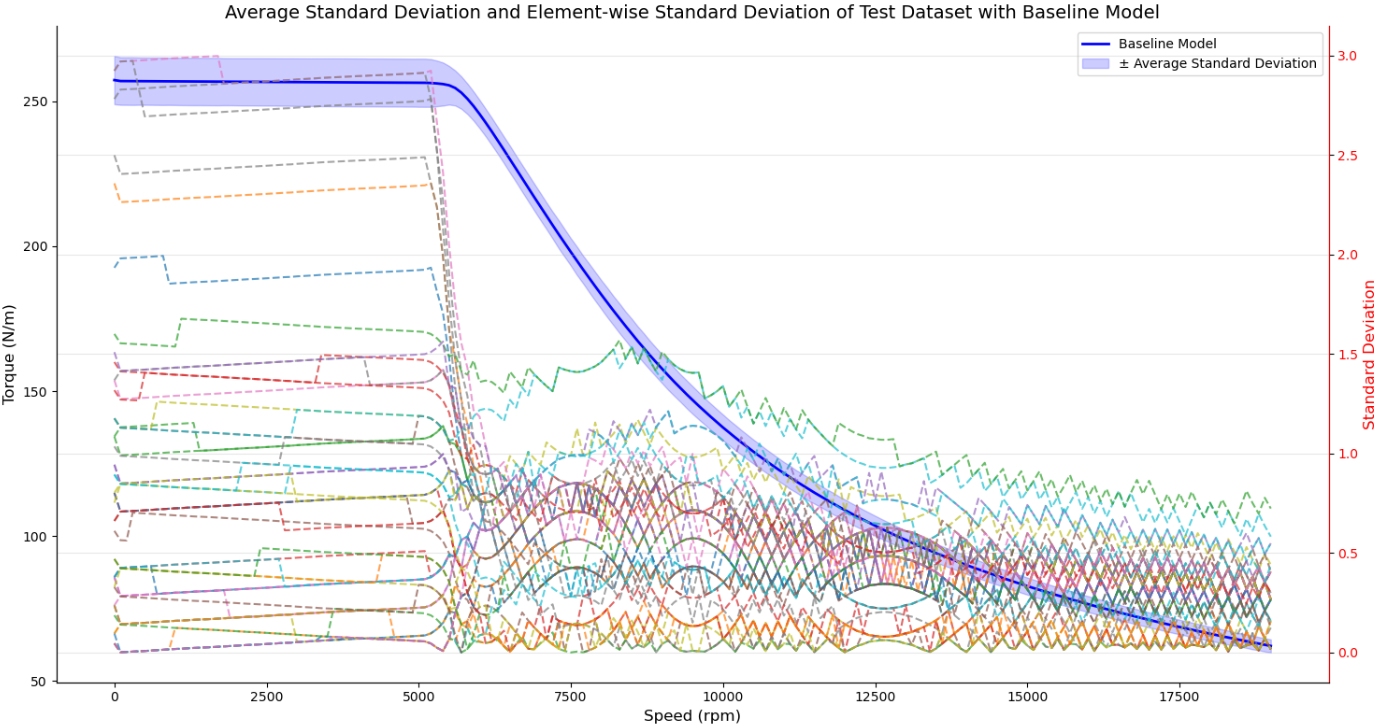
\includegraphics[width=1\textwidth]{./ReportImages/stddev_y1.png} 
    \caption{Standard Deviation of 2D KPI(ETA) Targets} 
    \label{fig:Standard Deviation of 3D KPI(ETA) Targets}
\end{figure}

From the above plot, we can conclude that the curve is relatively constant for 1/4 of the curve after which it is relatively monotonically decreasing.
This finding is critical for how we modelled the loss regularization for the target. It will be further elaborated in the Section \S\ref{sec:Loss Regularization for 2D KPI}


\subsection{Deep Dive into the \ac{3D} KPI(ETA Curve)}\label{sec:Deep Dive into 3D KPI}
As the target values Mgrenz and ETA grids are not provided with the correct dimensions we have an additional step which takes the maximum torque value from the Mgrenz grid and create a similar grid ranging from -maximum torque to maximum torque. \\
We then choose only the rows corresponding to this range from the actual MM grid supplied and the same row indices is used to retrieve the ETA grid. \\
This step ensures that we grant the model the correct dimensions of the ETA grid based on Torque curve and predict likewise.\\


\begin{figure}[H]
    \centering
    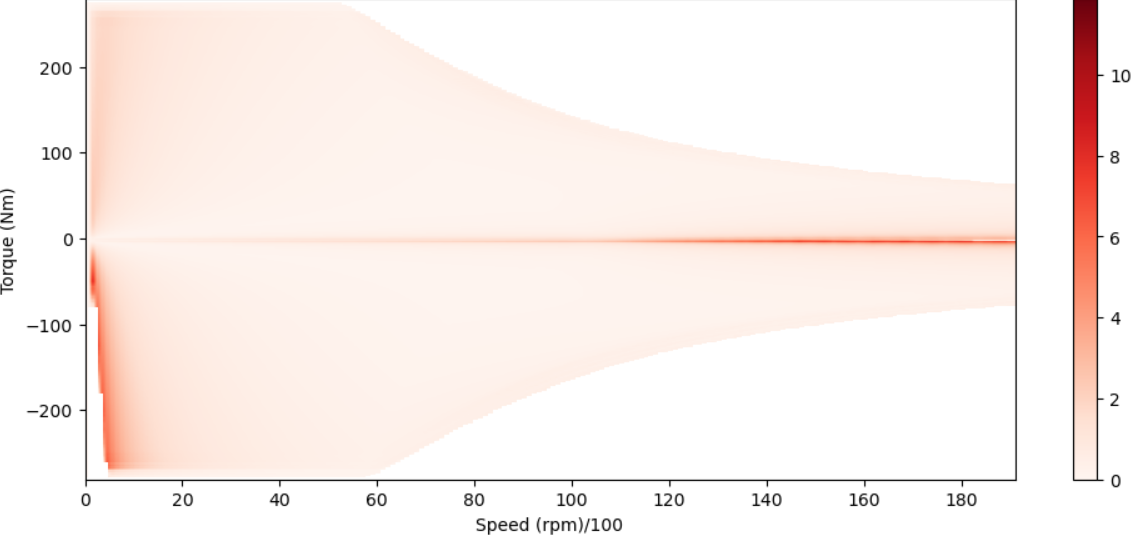
\includegraphics[width=1\textwidth]{./ReportImages/stddev_y2.png} 
    \caption{Standard Deviation of 3D KPI(ETA)} 
    \label{fig:Standard Deviation of 3D KPI(ETA)}
\end{figure}

More apparent below :

\begin{figure}[H]
    \centering
    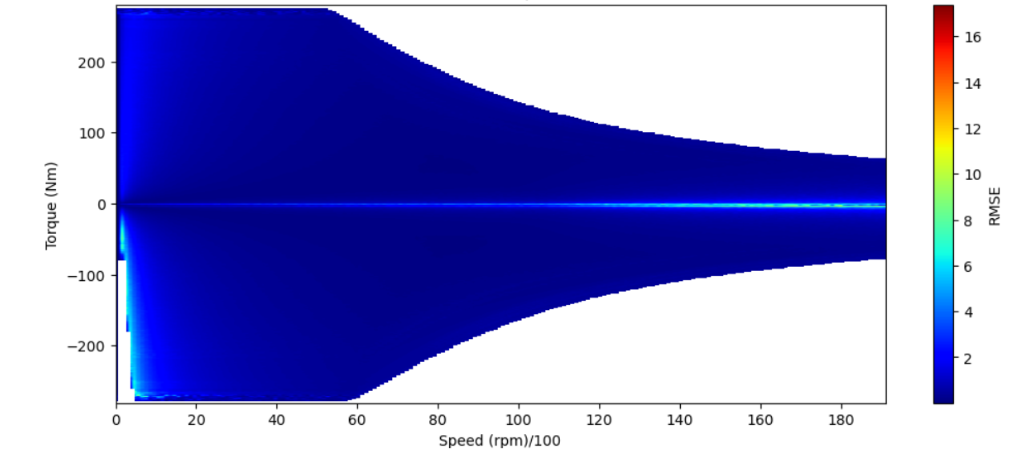
\includegraphics[width=1\textwidth]{./ReportImages/colorful_stddev_y2.png} 
    \caption{Standard Deviation of 3D KPI(ETA)} 
    \label{fig:Standard Deviation of 3D KPI(ETA)}
\end{figure}

From our analysis of the above plots on the standard deviation of the ETA grids from the test dataset, we notice that the data shared was faulty in the ETA corresponding to negative torque values.
As these are FEM simulations, it is probably an effect of a post processing step taken by the Motor builder.
The ETA grid corresponding to negative torque values when motor is in generating mode is not the replica as how it is for positive torque values when motor is in monitoring mode. 
This is evident from low speed high torque distribution area where we can see NAN values across the test dataset\\

Additionally the ETA grid envelope is completely dependent on its equivalent torque curve. The area beneath the boundary of which is looked into by the \ac{EM} manufacturers to determine the car's efficiency in the operating cycle.

From the plots received we find the ETA grid does not only cover the area within the torque curve but also a slightly exaggerated area typically in the portion where the 1/4 where the curve starts to monotonically decrease.
To ensure that out model is not tricked into assuming predictions for this extra area we extact the grid to be of the same shape as that of its curve.
This is a step also done as part of data post processing to be further overed in Section BLAH CITE. \\

Based on this finding, we have decided to only consider the ETA grid in monitoring mode for predictions and mirror the same to replicate the efficiency when it is in generating mode.\\

As reading the files take up a lot of time and compute, we read the files as a onetime job at the start and store them into pythonic objects for faster access in the future.\\
Both the input and target values for 1st \ac{KPI} is stored locally as pandas dataframe .csv files whereas the 2nd \ac{KPI} is stored as separate csv files per variant considering it is in the form of a \ac{2D} array.\\
The csv files are then concatenated and stored into a numpy array conserving dimensionality by padding nan values to match dimensionality of the grid corresponding to the torque curve with the largest torque value.\\
In our case the value is 561 but this is subject to change as we receive more data and can be overridden by the user.\\
The array is then saved locally as a .npy file for easy access and loading during training.\\

The input data consists of about 1500 examples mostly from the Double V Magnet Topology (and about 3 examples each for the other 2 topologies).\\ 

\section{Scaling}\label{sec:Scaling}

We have used Standard Scaling for the input and both the outputs.

The Scaling is formulated as shown below :

\begin{equation}
    \text{z} = \frac{x - \mu}{\sigma}
    \label{eq:Standard Scaling}
\end{equation} 

\textit{where
        \begin{itemize}
            \item x : Input
            \item $\mu$: : Mean
            \item $\sigma$: : Standard Deviation
        \end{itemize}
}

both Mean and Standard deviation are calculated across columns. This is attributed to the fact we have columns with different ranges for the input. 
Meanwhile the torque curve and the ETA grid are flattened to be 1D and thus have only 1 column.

We then removed scaling for the targets because these donot enter the model but is only used for loss calculation.
With lower learning rates and higher epochs, we see the model's y1 performing better than with scaling.
A plausible reason could be since the y1 targets are integers typically but we use torch tensor as it is a regression problem. This misleads the model with scaled targets to lose precision by generating within the full capacity of float tensors.
However without scaling, we observe the model spits out integers itself even when the datatype is still torch tensor. This inturn fixes the y1 earlier problem of having fluctuations in the curve.
Furthermore it now eliminates the need for regularizing the Y1 targets as predictions are as per target a smooth decreasing curve.\\

Additionally, the nan values in y2 are handled by masking before loss calculation as is defended in Section CITE Loss function
Initially before masking y2's nans we try to set it as an incredibly high value - but this resulted in poor predictions as the model must have been confused and tried to increase its spread of predictions to cover this value and so all true values were also predicted to be close to this dummy value--with scaling

\section{Dataset splitting}\label{sec:Dataset splitting}

We have also split the dataset to have about 50 samples for test and the remaining is used for 5 fold cross validation with 80:20 split for training and validation. \\
The reason we have a separate test dataset from the validation is to ensure that there is no data leakage as we donot want to overfit the testdataset with the hyperparameters we choose during training. \\

Within 5 folds, we expect to cover most grounds on training and have good monitoring on the model's performance for each fold.
We also choose the best hyperparameters that fits with our work on analysing the logs.
The best performing model is then chosen from the folds based on the model which has a combination of least aggregated loss for both outputs and scores for each output which are closest to 0.


\chapter{Graph Modelling} 

We intended to model our problem as a Graph and solve using Graph Neural Networks. 
We presume this will be a more clever way of representing our usecase in comparision to tabular data..
The idea was to make use of the Graph dynamics in our usecase and aggregate features that are semantically similar.
The main method of aggregating information within the nodes of a Graph is through Message Passing.
Graph Neural Networks can be broadly classified as :
Homogeneous GNN
Here the nodes and edges are of the same type. Message passing is done across the neighbouring nodes and edges over hops until it learns a representation equivalent from its neighbours
Heterogeneous GNN
Wherein the node and edge are of different types. Here message passing is conditioned on the node and edge type thus allowing the flow of information to be more controlled.

Standard Message Passing GNNs (MP-GNNs) can not trivially be applied to heterogeneous graph data, as node and edge features from different types can not be processed by the same functions due to differences in feature type. 
A natural way to circumvent this is to implement message and update functions individually for each edge type. 
During runtime, the MP-GNN algorithm would need to iterate over edge type dictionaries during message computation and over node type dictionaries during node updates.

\section{Data Preprocessing for \ac{GNN}}\label{sec:Data Preprocessing for GNN}


\textbf{Node types}

\begin{enumerate}
    \item \textbf{General}
    
    \begin{itemize}
        \item General parameters:
        \[
            r = \{r_{i}\} \quad \forall i \in \{a, r, o\} 
        \]
        
        \textit{where:
        \begin{itemize}
            \item $r_{a}$: Outer Radius of the Stator
            \item $r_{r}$: Outer Radius of the Rotor
            \item $r_{o}$: Center of the \ac{EM}
        \end{itemize}}
    \end{itemize}
    
    \item \textbf{Stator}
    
    \begin{itemize}
        \item Slot windings:
        \[
            sw = \{s_{i}w_{j}\} \quad \forall i \in \{1, \dots, QSim\}, \quad \forall j \in \{1, \dots, N\} 
        \]
        
        \item Slots:
        \[
            s = \{s_{i}\} \quad \forall i \in \{1, \dots, QSim\}
        \]

        \textit{where
        \begin{itemize}
            \item Qsim : Count of slots in the Stator
            \item N : Count of copper windings per slot
        \end{itemize}}
    \end{itemize}
    
    \item \textbf{Rotor}
    
    \begin{itemize}
        \item Magnet Flux Barriers:
        \[
            v = \{v_{ij}\} \quad \forall i \in \{1, \dots, T\}, \quad \forall j \in \{1, \dots, V\}
        \]
        
        \item Magnets:
        \[
            vm = \{v_{i}m_{j}\} \quad \forall i \in \{1, \dots, T\}, \quad \forall j \in \{1, \dots, V\}
        \]
        \textit{where
        \begin{itemize}
            \item T : Topology type of the \ac{EM}
            \item V : Type of Magnet
        \end{itemize}
        As Valeo only manufactures Double V magnets we consider it to be 2}
    \end{itemize}    
    
\end{enumerate}

\textbf{Edge types}

\begin{enumerate}
    \item \textbf{Angle} \\
    \textbf{Relevant Paths}
    \[
    vm--vm = \{ v_{i_{1}}m_{j_{1}} - v_{i_{2}}m_{j_{2}} \}
    \forall i_1, i_2 \in \{1, \dots, T\}, \quad \forall j_1, j_2 \in \{1, \dots, V\} \mid
    i_1 = i_2, \quad j_1 \neq j_2
    \]

    \textbf{angle}=vm-vm

    \item \textbf{Distance} \\
    \textbf{Relevant Paths}
    % \[
    %     v-v = \{ (v_{i_1 j_1} - v_{i_2 j_2}), \forall i_1, i_2, j_1, j_2 \in \{1, \dots, T\} \mid i_1i_2 \neq j_1j_2 \ \land (i_1 == i_2 \lor j_1 == j_2) \}
    % \]
    \[
        vi--vi = \{v_{i j_1} - v_{i j_2}\}, \forall i \in \{1, \dots, T\}, \forall j_1, j_2 \in \{1, \dots, V\} \mid  j_1 \neq j_2
    \]
    \[
        vi--vj = \{v_{i_1 j} - v_{i_2 j}\}, \forall i_1, i_2 \in \{1, \dots, T\}, \forall j \in \{1, \dots, V\} \mid  i_1 \neq i_2
    \]
    \[
        v--vm = \{v_{i j} - v_{i}m_{j}\} \forall i  \in \{1, \dots, T\}, \quad \forall j \in \{1, \dots, V\}
    \]
    \[
        v--rr = \{v_{i j} - r_{r}\}, \forall i, j  \in \{1, \dots, T\}
    \]
    \[
        o--r = \{ (o - r_{r}), (o - r_{a})\}
    \]
    \[
        rr--s = \{r_{r} - s_{i}\}, \forall i  \in \{1, \dots, QSim\}
    \]
    \[
        s--sw = \{s_{i} - s_{i}w_{j}\}, \forall i  \in \{1, \dots, QSim\}, \forall j  \in \{1, \dots, N\}
    \]
    \[
        s--ra = \{s_{i} - r_{a}\}, \forall i  \in \{1, \dots, QSim\}
    \]
    \[
        sw--sw = \{s_{i}w_{j_1} - s_{i}w_{j_2}\}, \forall i  \in \{1, \dots, QSim\}, \forall j  \in \{1, \dots, N\} \mid (j_1 == j_2-1)
    \]

    \textbf{distance} = vi--vi + vi--vj + v--vm + v--rr + o--r + rr--s + s--sw + s--ra + sw--sw

\end{enumerate}

\textbf{Node Features}

\begin{enumerate}

    \item \textbf{v} = \{lmsov, lth1v, lth2v, r1v, r11v, r2v, r3v, r4v, rmt1v, rmt4v, rlt1v, rlt4v, hav\}

    \item \textbf{vm} = \{mbv, mhv, rmagv\}

    \item \textbf{r} = \{r\}

    \item \textbf{s} = \{b\_nng, b\_nzk, b\_s, h\_n, h\_s, r\_sn, r\_zk, r\_ng, h\_zk\}

    \item \textbf{sw} = \{bhp, hhp, rhp\}
\end{enumerate}

\textbf{Path Features}

\begin{enumerate}

    \item \textbf{vm--vm} = \{deg\_phi\}

    \item \textbf{vi--vi} = \{dsm, dsmu\}

    \item \textbf{vi--vj} = \{amtrvj-amtrvi\}

    \item \textbf{v--vm} = \{lmav, lmiv, lmov, lmuv\}

    \item \textbf{v--r} = \{amtrv, dsrv\}
    
    \item \textbf{o--r} = \{r\}

    \item \textbf{rr--s} = \{airgap\}

    \item \textbf{s--sw} = \{dhphp\}
    
    \item \textbf{sw--sw} = \{dhpng\}
    
    \item \textbf{s--ra} = \{r\_a-(r\_i + h\_n + h\_zk)\}
    
\end{enumerate}
The heterogeneous graph that was constructed earlier is as below:
\begin{figure}[H]
    \centering
    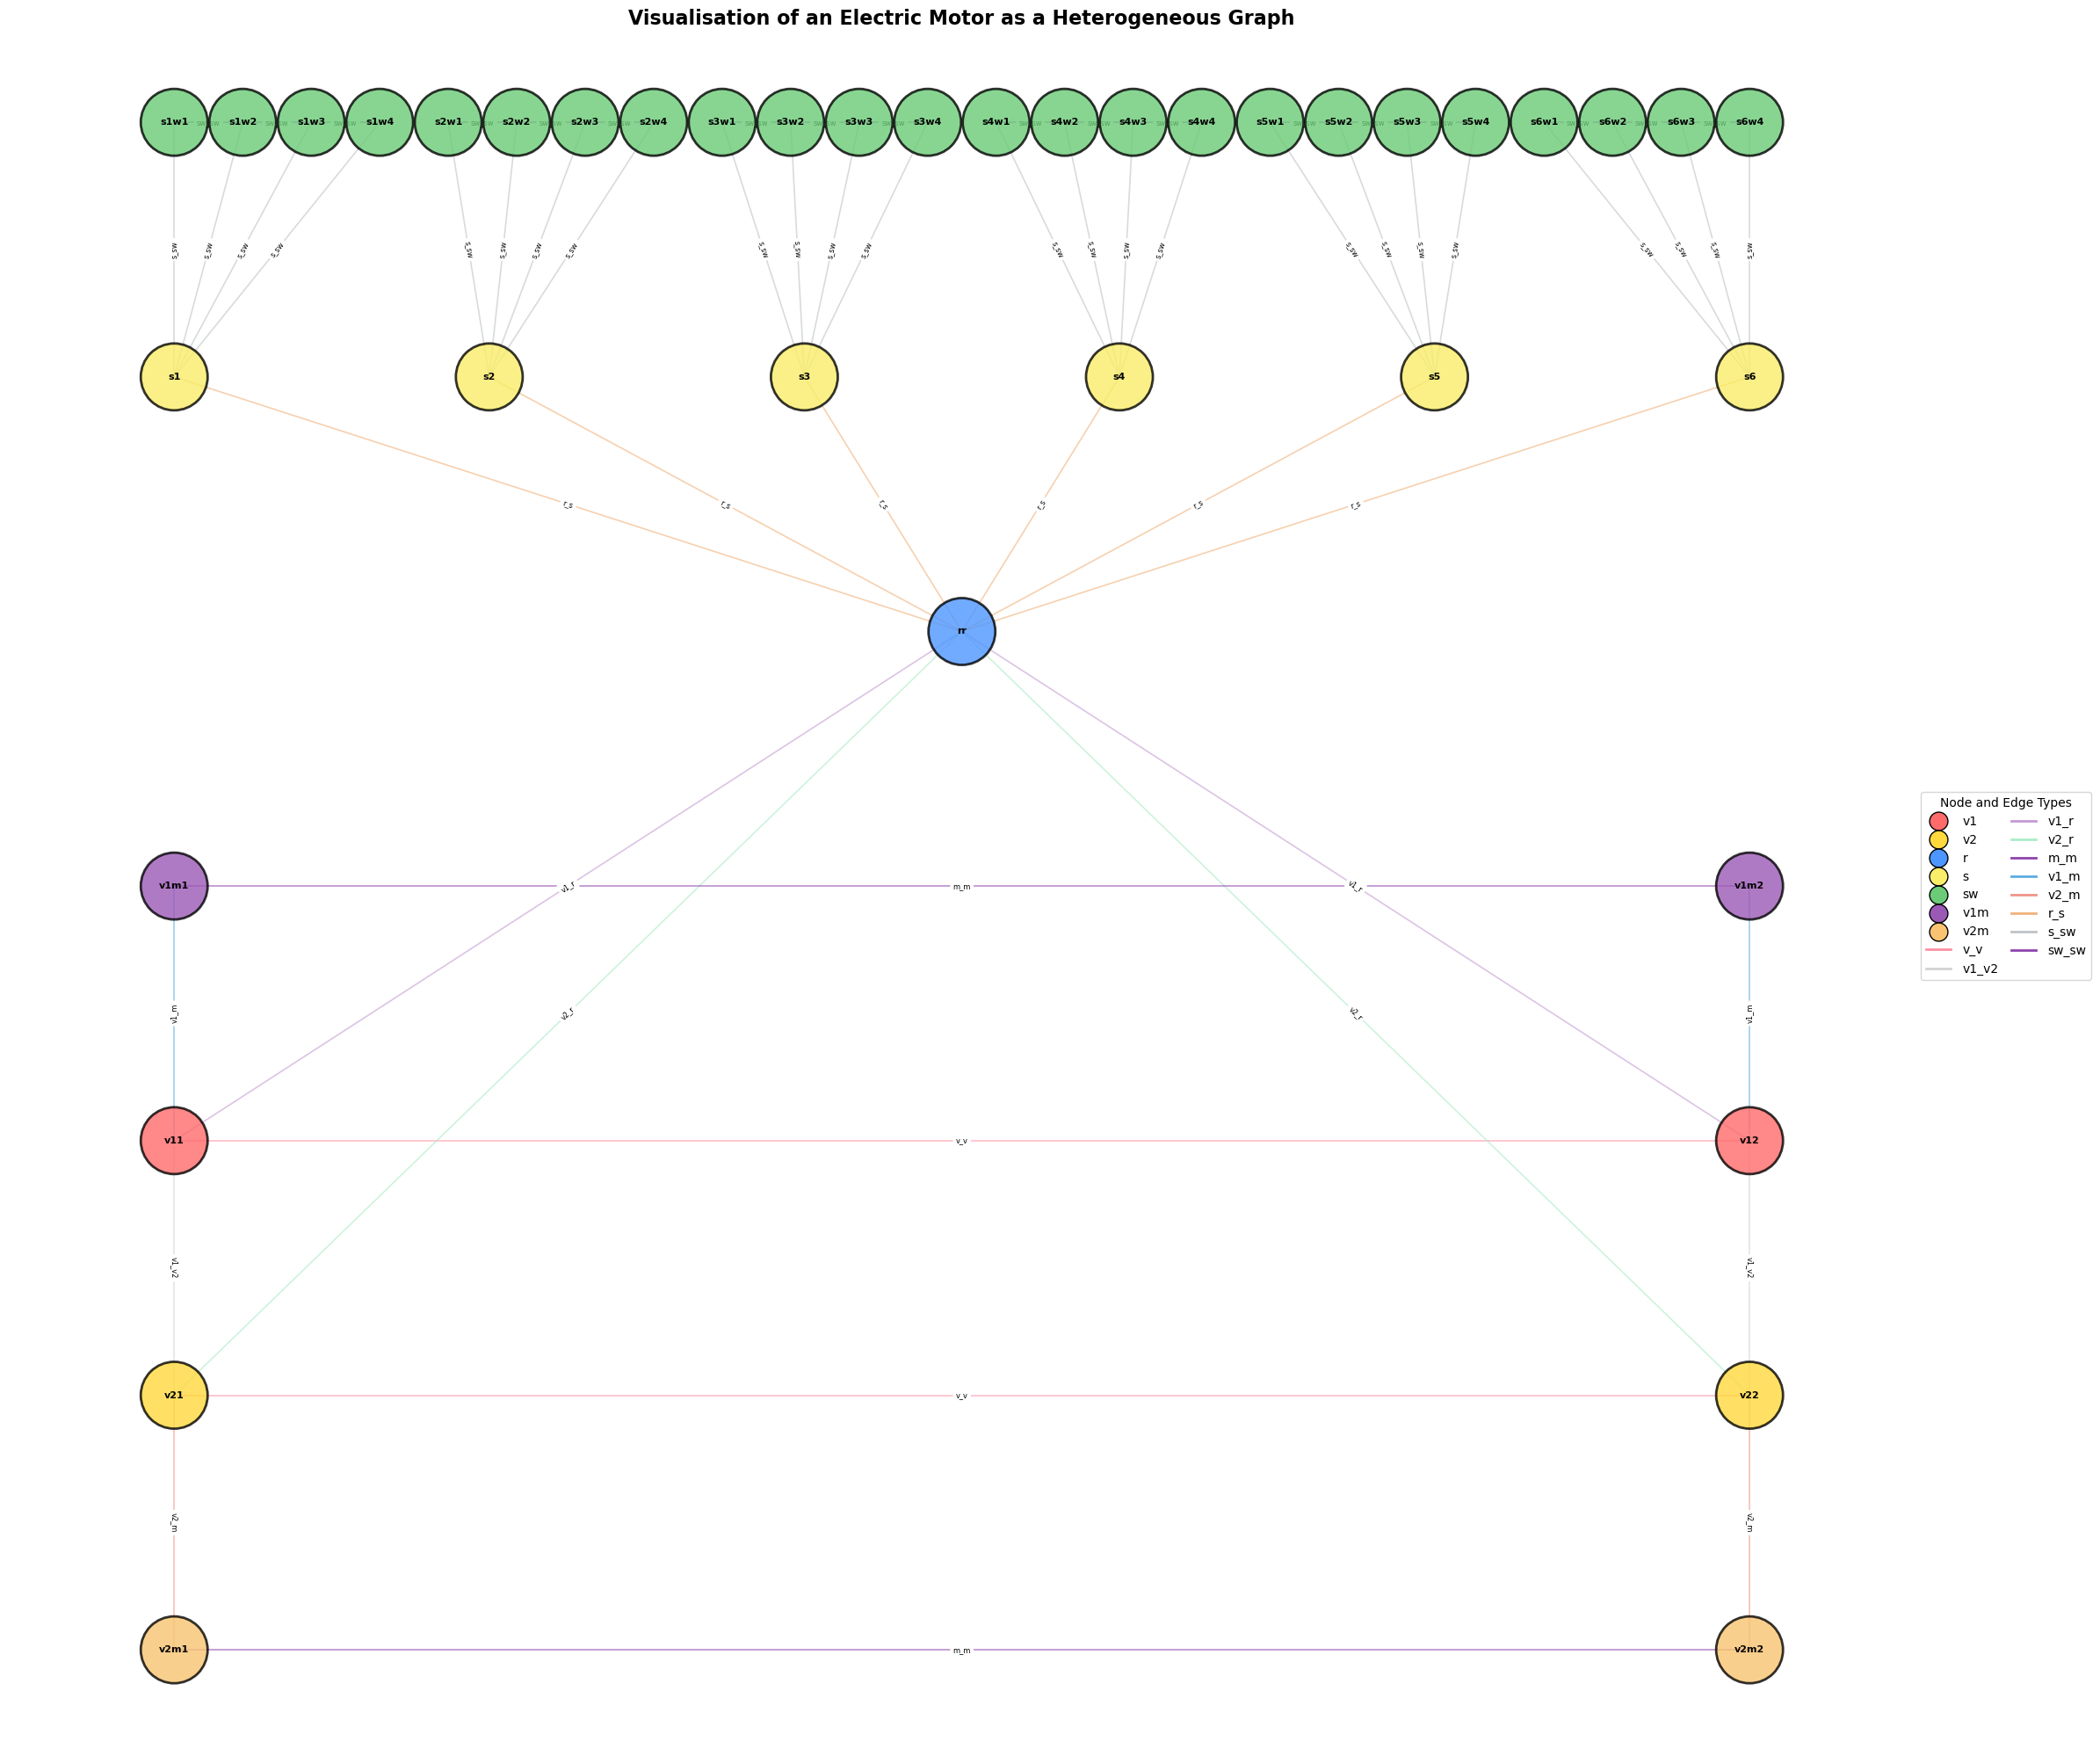
\includegraphics[width=0.9\textwidth]{./ReportImages/graph.png} 
    \caption{HetGraph}
    \label{fig:Graph}
\end{figure}


\section{Heterogeneous \ac{GNN} Model}\label{sec:Heterogeneous GNN Model}

We find the heterogeneous graph to be most apt for our use case with its different node and edge types as it preserves both the structural and semantics of our data. \\
This property is crucial in modelling our use case as we will then have similar node-edge types per topology. \\
In addition the count of certain parameters with the motor such as stator poles with its corresponding slot and rotor magnets is made more comprehendable to the model having new nodes and edges whereas for the \ac{MLP} architecture this information is represented only as a number in yet another column. \\
Heterogeneous \ac{GNN} generally work by having separate non linear functions convolve over each edge type during message computation and over each node type when aggregating the learned information. \\
 
\newpage 
\chapter{Modelling \& Evaluation}

Since we aim to predict continuous vector values, we model this task into a regression problem
As a baseline, we first train a \ac{MLP} on the tabular representation of the data and work on it further to do the same with a heterogeneous \ac{GNN}.

\section{\ac{MLP} Model}\label{sec:MLP Model}

For the \ac{MLP} model, we use a single model with input features corresponding to all the features in the tabular topology invariant representation of the data.\\
The model architecture is build to predict both the \ac{2D} and \ac{3D} \ac{KPI}s by having 2 separate output layers for each of the \ac{KPI}s. \\
Since the \ac{2D} \ac{KPI}'s targets are relatively learnable than that of the \ac{3D} \ac{KPI}'s targets we have experimented with fewer feed forward layers in the former than in the latter.
RELU layers were also added in between to serve as the activation function and produce non-linearities in the model. \\
Dropout layers ensure that not all neurons in each layer are used up during training to prevent the model from memorizing the data and hence overfitting.
Batch normalisation layers are used to normalize the input to the next layer and hence speed up the training process.\\

Th model architecture is designed to have 2 fully connected layers with RELU as an activation function and a 1D batch normalisation layer with a dropout layer for the 1st output.\\
We have also used a dropout percentage of 0.2 to ensure the model does not overfit the data by dropping out 20 percent of the neurons in the layer.
Although the targets for the first output are an array of integer values, we use the float tensor and not integer tensor to represent the data else it would become a classification problem and not a regression problem as it should be. \\
For the second output we have 5 fully connected layers with RELU as an activation function and dropout and \ac{2D} batch normalisation for each layer.\\

The below figure gives an outline on how the MLP Model architecture is designed.

\begin{figure}[H]
    \centering
    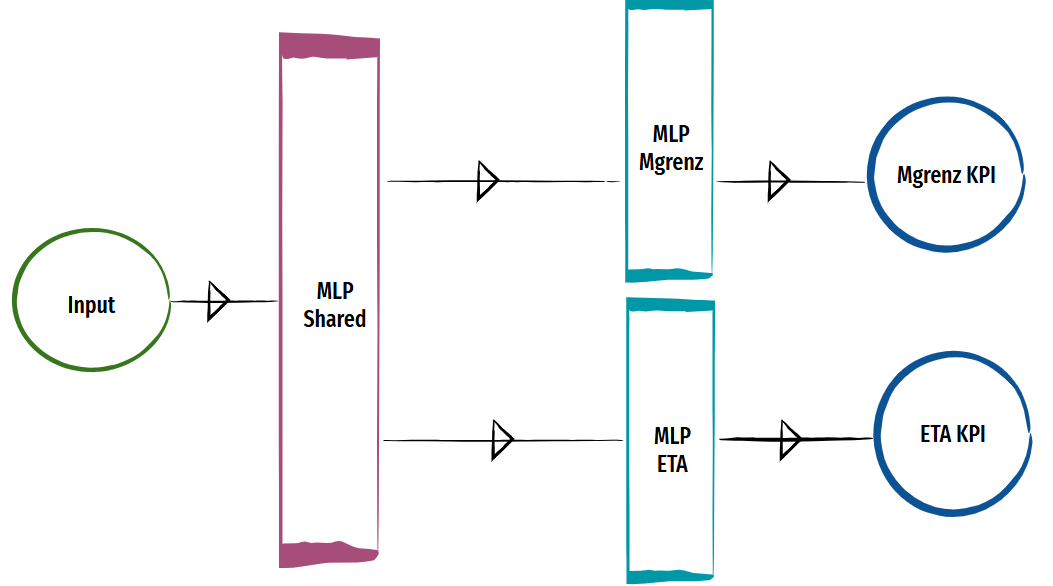
\includegraphics[width=1\textwidth]{./ReportImages/mlp_architecture.png} 
    \caption{MLP Model Architecture}
    \label{fig:MLP Model Architecture}
\end{figure}

\section{Loss Functions}\label{sec:Loss Functions}
The \ac{MSE}loss is the loss function used for our problem with the intention that the losses are minimized. We have adopted 2 methodologies to regularize the loss one each for the \ac{2D} and \ac{3D} \ac{KPI}.

\subsection{Loss Regularization for \ac{2D} \ac{KPI}(Torque curve)}\label{sec:Loss Regularization for 2D KPI}

The \ac{MSE} loss for the \ac{2D} \ac{KPI} is formulated as shown below :
% Mean Squared Error (\ac{MSE}) Loss for 2D KPI
\begin{equation}
    \text{Y1 Loss} = \frac{1}{n} \sum_{i=1}^{n} \frac{1}{h} \sum_{j=1}^{h} (y_{ij} - \hat{y}_{ij})^2
    \label{eq:Y1 Loss}
\end{equation} 

\textit{where
        \begin{itemize}
            \item n : \ac{EM} samples
            \item h : dimensionality of 1D vector
        \end{itemize}
}


To smoothen out the curve for the \ac{2D} \ac{KPI}(Torque curve) we apply a loss regularisation factor to take into account before backpropagating it the model during training. \\
We observed the curve inherently follows a decreasing pattern CITE AGAIN::COULD BE A KNOWN FACT:::and hence using this knowledge penalize the loss for non-decreasing values within each prediction. \\
CITE!!!!If the electromagnetic coil is enabled by the commutator for the time span t3, the (almost) maximal current is running through it's loops and the (almost) maximal magnetic field strength is generated. The (almost) maximal torque is acting on the rotor. If the time span is shortened to t2 by increasing rotational speed, a slightly lower torque is acting, because the current through the coil is decreasing slightly. When reducing the time span to t1, the coil gets disconnected from the input voltage even though just half the maximum current is reached. Accordingly the torque decreases significantly:
%[https://homofaciens.de/technics-electric-motors-torque-curve_en.html]

% Regularization Term

\begin{equation}
\text{Y1 Loss Regularization} = \frac{1}{n} \sum_{i=1}^{n}\frac{1}{h-1} \sum_{j=1}^{h-1} \left(\text{ReLU}(\hat{y}_{i{j+1}} - \hat{y}_{ij})\right)^2
\label{eq:Y1 Loss Regularization}
\end{equation} 

\textit{where
\begin{itemize}
    \item RELU : Activation Function
\end{itemize}
}

Theoretically, we would expect the model to generate better predictions but on closer observation we notice the curve is still not smooth. \\
A reason to attribute this could be the model's incapability to infer that loss decrease depends on not just the prediction and target values but also within prediction values.
Our deduction is that a single value calculated for the entire curve may not be sufficient to regularize this loss as we imagined. \\

A reason to attribute this could be the model's struggle to attempt to generate the next point in the curve to be smaller than the previous point yet also for the further point in addition to making sure the \ac{MSE} is calculated accurately.
Our hypothesis is this loss regularization creates a tug of war between the \ac{MSE} loss and the regularization term when predicting the whole curve and hence the ever fluctuating curve being generated.\\


\subsection{Loss Customization for \ac{3D} \ac{KPI}(Efficiency Grid)}\label{sec:Loss Customization for 3D KPI}

The \ac{MSE} loss is calculated for the \ac{3D} \ac{KPI} is formulated as shown below :
% Mean Squared Error (\ac{MSE}) Loss for 3D KPI
\begin{equation}
\text{Y2 Loss} = \frac{1}{n} \sum_{i=1}^{n} \frac{1}{w} \frac{1}{h} \sum_{j=1}^{w} \sum_{k=1}^{h} \left( M_{ijk} \cdot y_{ijk}) - (M_{ijk} \cdot \hat{y}_{ijk})\right)^2
\label{eq:Y2 Loss}
\end{equation}

\textit{where
\begin{itemize}
    \item $M_{ijk}$ : Mask matrix
    \begin{equation*}
        M_{ijk} = \begin{cases}
            1 & \text{if } y_{ijk} \neq \text{nan } \\
            0 & \text{if } y_{ijk} = -1
            \end{cases} \\
    \label{eq:Mask matrix}
    \end{equation*}
    \item w : 1st dimension of \ac{3D} vector
    \item h : 2nd dimension of \ac{3D} vector
\end{itemize}
}

The ETA Grid is a \ac{3D} plot of real numbers ranging between 0 and 100.NEED TO CITE...EVEN IF IT IS A KNOWN FACT We noticed in some portions of the grid, the plot not visible as it had nan values.\\
As ANN cannot be trained to predict NAN values we have a binary mask constructed such that values corresponding to -nan in the target have value 0 and all other values as 1. The mask is then multiplied with the prediction. 
Furthermore the mask is used to replace nan values in target with 0 as multiplying a nan value with 0 results in yet another nan value. This would cascade into nan loss calculation. \\
After this step, the \ac{MSE} loss is calculated and backpropagated. \\
Mathematically, this process can be expressed as above

This formulation ensures that the -1 values (which replaced NaN values in the grid) are ignored in the loss calculation, as they are multiplied by 0 in the mask.\\

It is a known fact that at 0 Torque, the corresponding efficiency values for the motor is 0.
To model this conception into our network, we have attempted to retrieve the center row of our ETA grid and the values it consists finally determine the violation count.
We formulate is mathematically as below:


\begin{equation}
    \text{Y2 Loss Regularization} = \frac{1}{n} \sum_{i=1}^{n} \frac{1}{h} \sum_{k=1}^{h} |y_{i0k}|
   \label{eq:Y2_Loss_Regularization}
\end{equation}


We take the absolute values from the center row of the matrix else the loss would be negative and could negate with positive values. This would have a detrimental effect when calculating the loss


\begin{equation}
    \begin{split}
\text{Total Loss} = \text{Y1 Weight} \times (\text{Y1 Loss} + (\lambda_{\text{y1}} \times \text{Y1 Loss Regularization})) +\\
 \text{Y2 Weight} \times (\text{Y2 Loss} + (\lambda_{\text{y2}} \times \text{Y2 Loss Regularization}))
    \end{split}
    \label{eq:Total Loss}
\end{equation}

\textit{where
\begin{itemize}
    \item[]
       \begin{align*}
       \lambda_{\text{y1}} &: \text{Y1 Loss Regularization Weight}
       \end{align*}
    \item[]
       \begin{align*}
       \lambda_{\text{y2}} &: \text{Y2 Loss Regularization Weight}
       \end{align*}
    \item Y1 Weight : Y1 Loss Weightage 
    \item Y2 Weight : Y2 Loss Weightage
\end{itemize}
}

\section{Optimizer}\label{sec:Optimizer}

Adam optimizer is used for optimization as it is known to be computationally efficient and requires little memoryBLAH BLAH \\
The optimizer acts once the loss is backpropagated across training each batch of the dataset.\\
We have also experimented with a learning rate scheduler which reduced the learning rate exponentially by a gamma parameter to decay learning as training progresses across epochs.

\section{Evaluation Metrics}

The evaluation metrics we have considered for our regression problem is the root mean squared error. \\
The model with the least combined loss and prediction scores closest to 0 is ideal for our application. \\

\subsection{Evaluation Metrics for \ac{2D} \ac{KPI}}\label{sec:Evaluation Metrics for 2D KPI}

The y1 loss for the \ac{2D} \ac{KPI} is formulated as shown below :
% Evaluation metric (\ac{MSE}) Loss for 2D KPI
\begin{equation}
\text{Y1 score} = \frac{1}{n} \sum_{i=1}^{n} \sqrt{\frac{1}{h} \sum_{j=1}^{h} (y_{ij} - \hat{y}_{ij})^2}
\label{eq:Y1 score}
\end{equation}

\textit{where
        \begin{itemize}
            \item n : \ac{EM} samples
            \item h : dimensionality of 1D vector
        \end{itemize}
}

\subsection{Evaluation Metrics for \ac{3D} \ac{KPI}}\label{sec:Evaluation Metrics for 3D KPI}

The y2 loss for the \ac{3D} \ac{KPI} is formulated as shown below :
%  Evaluation metric (\ac{MSE}) Loss for 3D KPI
\begin{equation}
    \text{Y2 score} = \frac{1}{n} \sum_{i=1}^{n} \sqrt{\frac{1}{w} \frac{1}{h} \sum_{j=1}^{w} \sum_{k=1}^{h} (y_{ijk} - \hat{y}_{ijk})^2}
    \label{eq:Y2 score}
\end{equation}
    
    \textit{where
            \begin{itemize}
                \item n : \ac{EM} samples
                \item w : 1st dimension of 3D vector
                \item h : 2nd dimension of 3D vector
            \end{itemize}
    }

\section{Post Processing}\label{sec:Post Processing}

The mean and standard deviation from the train-validation datasets are applied to transform the test dataset to maintain uniformity on the predictions generated.
In the case of new files we first convert it into the tabular representation our model consumes and then do the scaling.\\
This is the reason why we preserve the same scalers used during training as we not only evaluate our dedicated test dataset but also for clients to use on demand. \\


The inverse scaling is formulated as shown below :

\begin{equation*}
\text{x} = \frac{z \times \sigma}{\mu}
\label{eq:Inverse Scaling}
\end{equation*}

\textit{where
        \begin{itemize}
            \item z : Scaled Input
            \item $\mu$: : Mean
            \item $\sigma$: : Standard Deviation
        \end{itemize}
}

Furthermore as part of post processing, we slice the 3D ETA grid to only contain the values within the predicted torque curve.

\newpage 
\newpage 

% Masking NAN values
\chapter{Experiments and Results}

\section{Experiments with \ac{MLP}}\label{sec:Experiments with MLP}

The hyperparameters were chosen via a random grid search and we finalized those that resulted in the ideal scores for both y1 ad y2 respectively.
The hyperparmaters for the model was tuned over observations of the model's performance across 5 fold cross validation training.\\
The splits are saved locally and can be used to later to ensure reproducibility.

\begin{table}[H]
    \centering
    \begin{tabularx}{1\linewidth}{|X|X|X|}
    \hline {\bf Hyperparameters} & {\bf Description} & {\bf Value}\\
    \hline 
    lr & Learning Rate & 0.00075 \\
    hidden\_sizes & Dimensionality of Hidden Layers& 256 \\
    lr\_gamma & Exponential Learning Rate Scheduler & 0.9 \\
    batch\_size & Batch Size & 72 \\
    epochs & Number of Epochs & 8 \\
    p & Dropout Probability& 0.2 \\
    lambda\_y1 & Y1 Loss Regularizer & 2.5 \\
    lambda\_y2 & Y2 Loss Regularizer & 1.5 \\
    w\_y1 & Weightage of Y1 Loss & 0.8 \\
    w\_y2 & Weightage of Y2 Loss & 0.2 \\
    \hline
    \end{tabularx}
    \caption{Hyperparameter Tuning}
    \label{tab:Hyperparameter Tuning}
\end{table}

Over the 5 folds, the model performance is observed to ensure its stability and the best performing model is saved to be loaded later for performance.
The criteria for choosing the best performing model is roughly estimated based on the least combined loss and the combined score closest to 0.\\
We chose \ac{Wandb} to log metrics from the training run and to monitor model performance across folds. \\
Below is the visualisation of the training and validation metrics for both \ac{KPI}s.\\

\begin{figure}[H]
    \centering
    \begin{minipage}[b]{0.3\textwidth}
        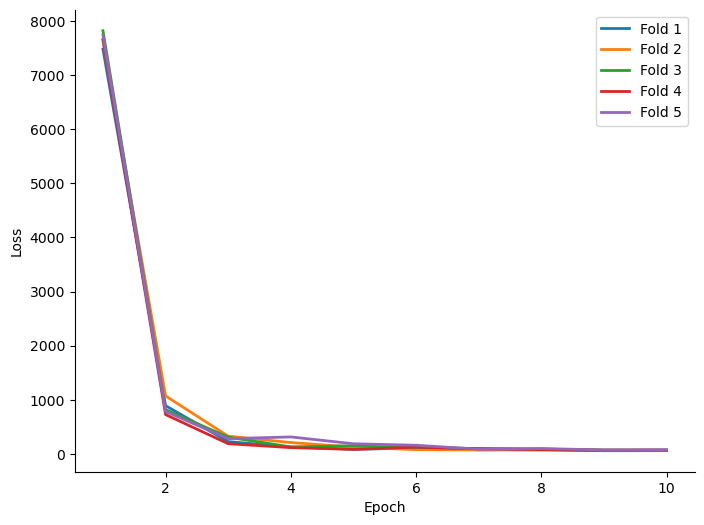
\includegraphics[width=\textwidth]{./ReportImages/train_loss.png}
        \caption{Aggregated Training Loss}
        \label{fig:Aggregated Training Loss}
    \end{minipage}
    \hfill
    \begin{minipage}[b]{0.3\textwidth}
        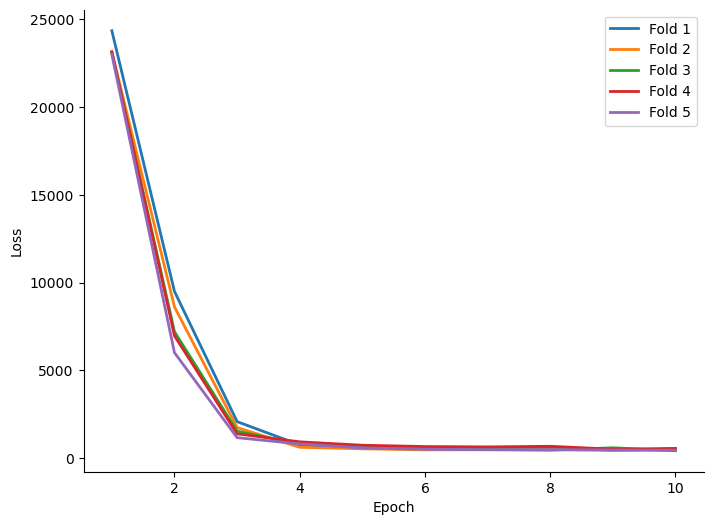
\includegraphics[width=\textwidth]{./ReportImages/train_loss_y1.png}
        \caption{Training Loss for Torque Curve}
        \label{fig:Training Loss for Torque Curve}
    \end{minipage}
    \hfill
    \begin{minipage}[b]{0.3\textwidth}
        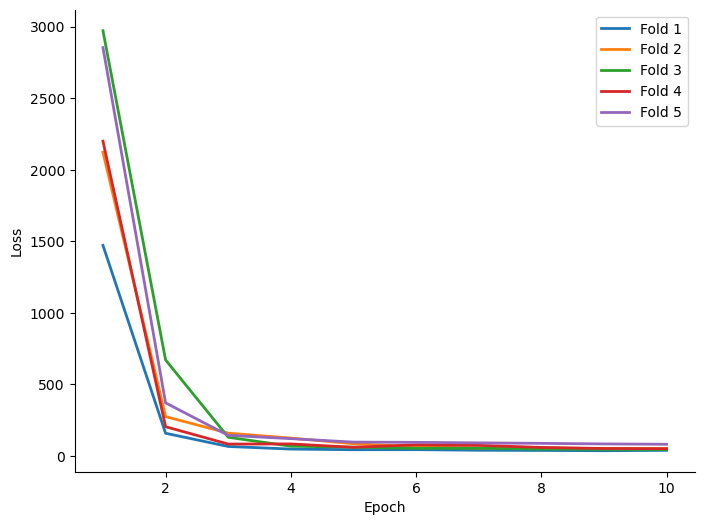
\includegraphics[width=\textwidth]{./ReportImages/train_loss_y2.png}
        \caption{Training Loss for ETA grid}
        \label{fig:Training Loss for ETA grid}
    \end{minipage}
\end{figure}

\begin{figure}[H]
    \centering
    \begin{minipage}[b]{0.3\textwidth}
        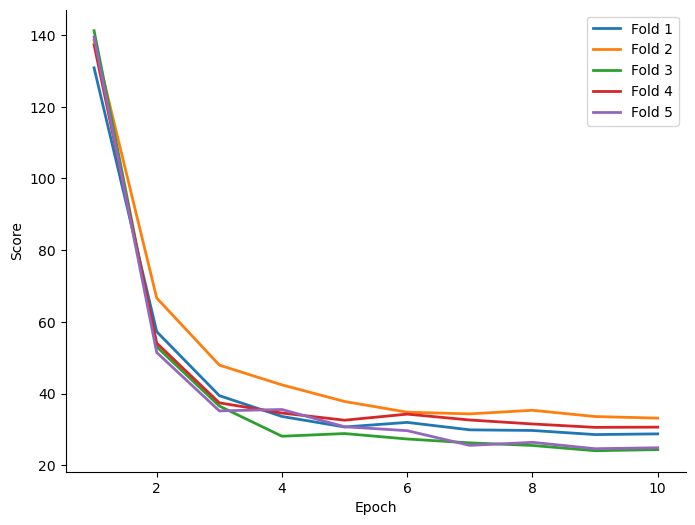
\includegraphics[width=\textwidth]{./ReportImages/train_score.png}
        \caption{Aggregated Training Score}
        \label{fig:Aggregated Training Score}
    \end{minipage}
    \hfill
    \begin{minipage}[b]{0.3\textwidth}
        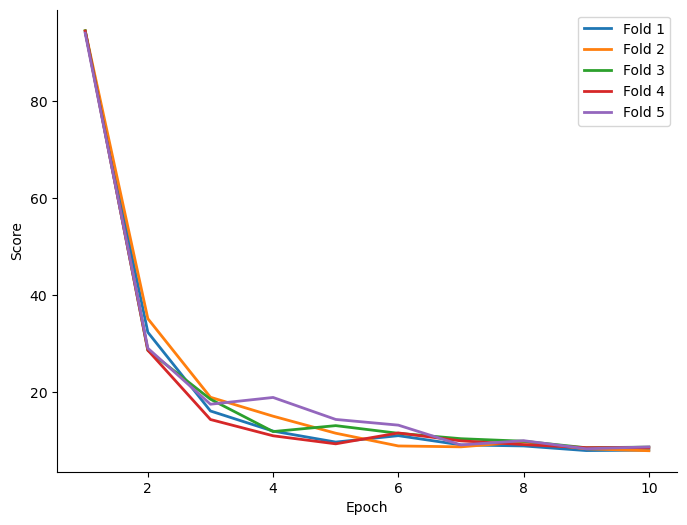
\includegraphics[width=\textwidth]{./ReportImages/train_score_y1.png}
        \caption{Training Score for Torque Curve}
        \label{fig:Training Score for Torque Curve}
    \end{minipage}
    \hfill
    \begin{minipage}[b]{0.3\textwidth}
        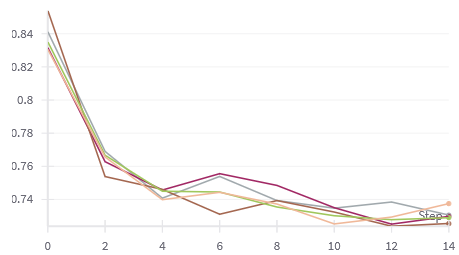
\includegraphics[width=\textwidth]{./ReportImages/train_score_y2.png}
        \caption{Training Score for ETA grid}
        \label{fig:Training Score for ETA grid}
    \end{minipage}
\end{figure}

From the training plots we see that the model has converged after having run for 10 epochs with a learning rate of 0.0075.

\begin{figure}[H]
    \centering
    \begin{minipage}[b]{0.3\textwidth}
        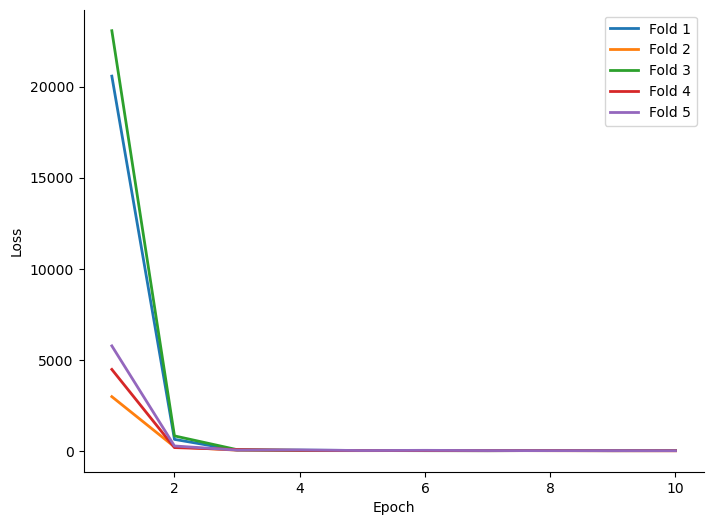
\includegraphics[width=\textwidth]{./ReportImages/val_loss.png}
        \caption{Aggregated Validation Loss}
        \label{fig:Aggregated Validation Loss}
    \end{minipage}
    \begin{minipage}[b]{0.3\textwidth}
        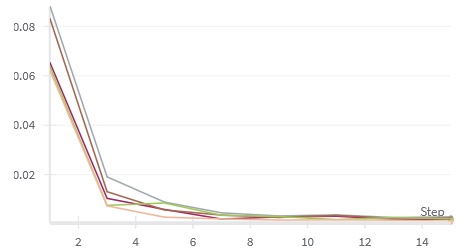
\includegraphics[width=\textwidth]{./ReportImages/val_loss_y1.png}
        \caption{Validation Loss for Torque Curve}
        \label{fig:Validation Loss for Torque Curve}
    \end{minipage}
    \hfill
    \begin{minipage}[b]{0.3\textwidth}
        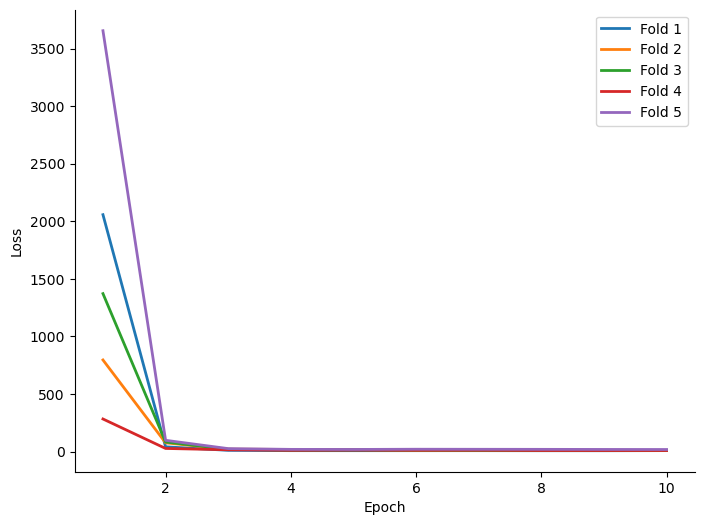
\includegraphics[width=\textwidth]{./ReportImages/val_loss_y2.png}
        \caption{Validation Loss for ETA grid}
        \label{fig:Validation Loss for ETA grid}
    \end{minipage}
\end{figure}

\begin{figure}[H]
    \centering
    \begin{minipage}[b]{0.3\textwidth}
        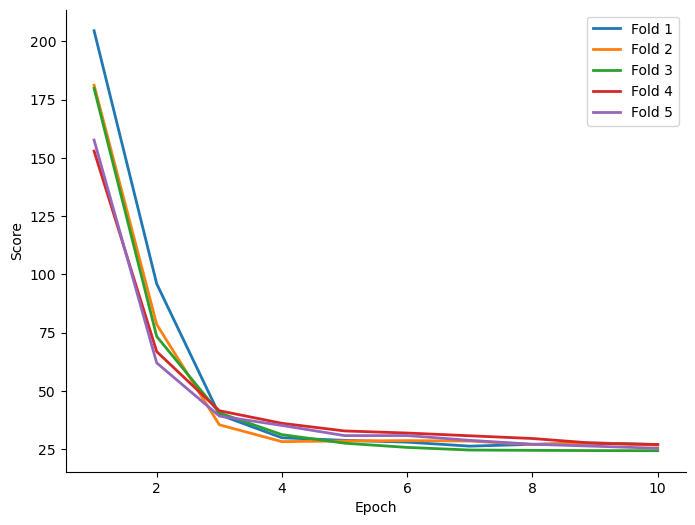
\includegraphics[width=\textwidth]{./ReportImages/val_score.png}
        \caption{Aggregated Validation Score}
        \label{fig:Aggregated Validation Score}
    \end{minipage}
    \begin{minipage}[b]{0.3\textwidth}
        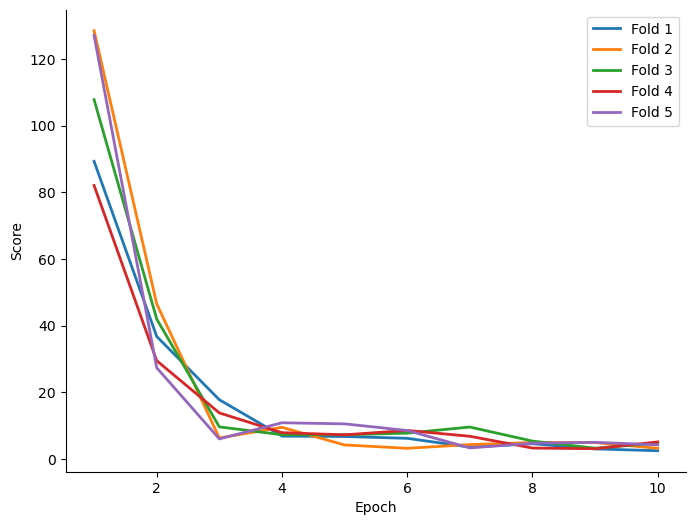
\includegraphics[width=\textwidth]{./ReportImages/val_score_y1.png}
        \caption{Validation Score for Torque Curve}
        \label{fig:Validation Score for Torque Curve}
    \end{minipage}
    \hfill
    \begin{minipage}[b]{0.3\textwidth}
        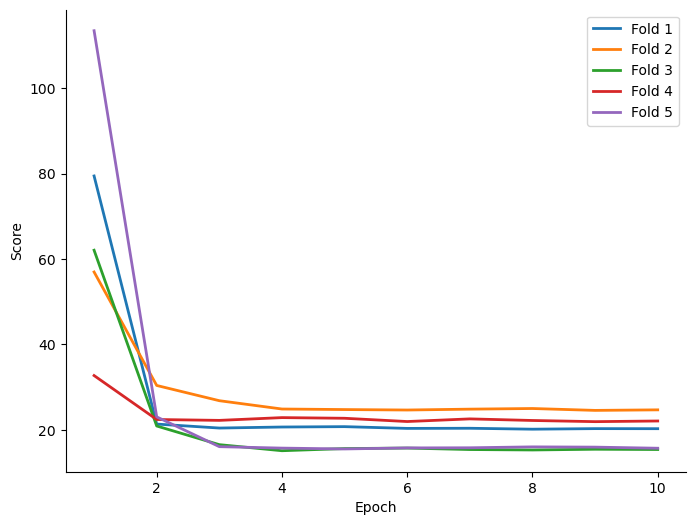
\includegraphics[width=\textwidth]{./ReportImages/val_score_y2.png}
        \caption{Validation Score for ETA grid}
        \label{fig:Validation Score for ETA grid}
    \end{minipage}
\end{figure}

We see a good fit of the model to the data with corresponding y1 and y2 scores approaching close to 1.
We have also enabled saving the trained model locally so it can be loaded on demand by the client to run inference.\\

We have narrowed down scoring to follow the below criteria:

\begin{table}[H]
    \centering
    \begin{tabularx}{1\linewidth}{|X|X|X|X|X|X|}
    \hline {\bf Scoring} & {\bf Excellent} & {\bf Very Good} & {\bf Good} & {\bf Average} & {\bf Bad}\\
    \hline 
    Y1 & 0-1 & 1-2 & 2-4 & 4-6 & \textgreater 6\\
    Y2 & 0-0.5 & 0.5-1 & 1-2 & 2-4 & \textgreater 4\\
    \hline
    \end{tabularx}
    \caption{Scoring Criteria}
    \label{tab:Scoring Criteria}
\end{table}


\section{Results with \ac{MLP}}\label{sec:Results with MLP}

The results of the \ac{MLP} model from inference is as below: \\

\subsection{2D Torque Curve Results with \ac{MLP}}\label{sec:2D Torque Curve Results with MLP}

\begin{figure}[H]
    \centering
    \includegraphics[width=1\textwidth]{./ReportImages/KPI2D_predictions.png} 
    \caption{MLP Training Results for 2D KPI(Mgrenz)} 
    \label{fig:MLP Training Results for 2D KPI(Mgrenz)}
\end{figure}

The Average RMSE and element wise RMSE for the test dataset performance with the \ac{MLP} is as below: \\

\begin{figure}[H]
    \centering
    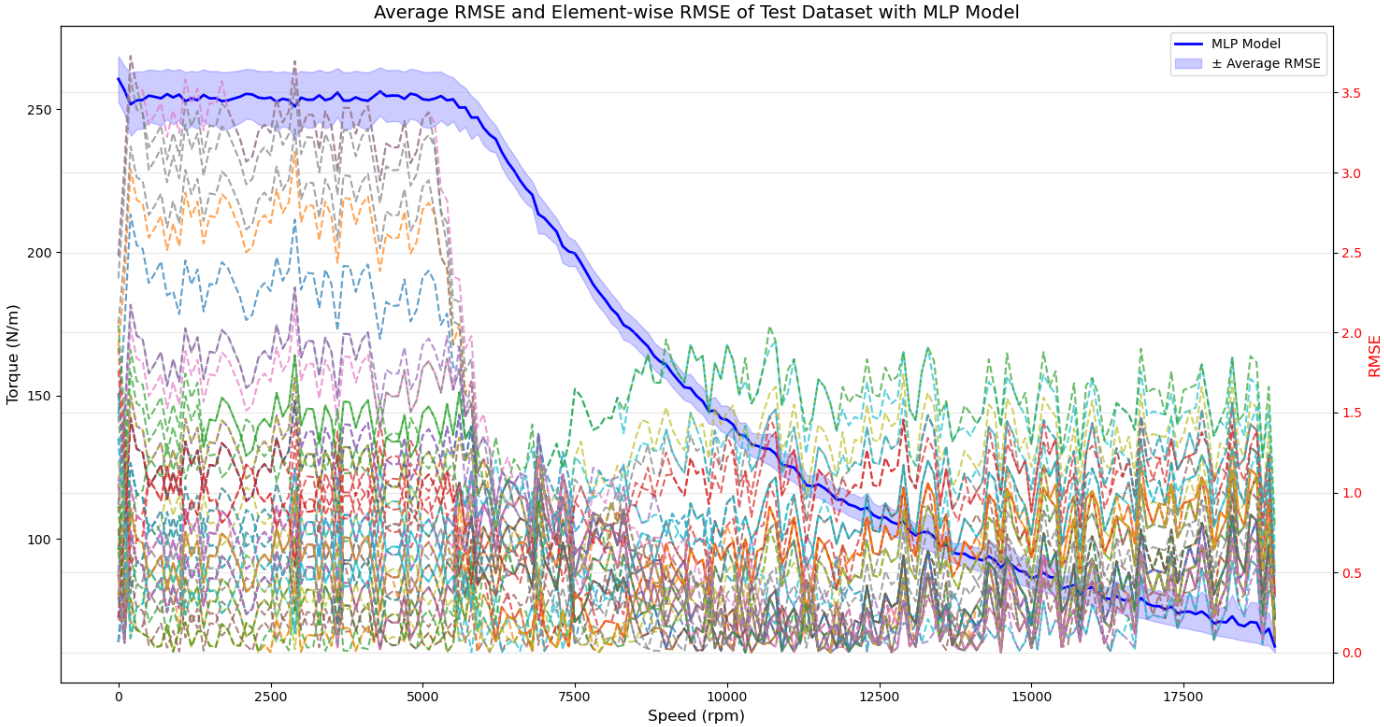
\includegraphics[width=1\textwidth]{./ReportImages/avgrmse_y1.png} 
    \caption{Test Dataset RMSE Evaluation for 2D KPI(Mgrenz)} 
    \label{fig:Test Dataset RMSE Evaluation for 2D KPI(Mgrenz)}
\end{figure}

We also have the score statistics of how the model performs over the test dataset.\\

\begin{figure}[H]
    \centering
    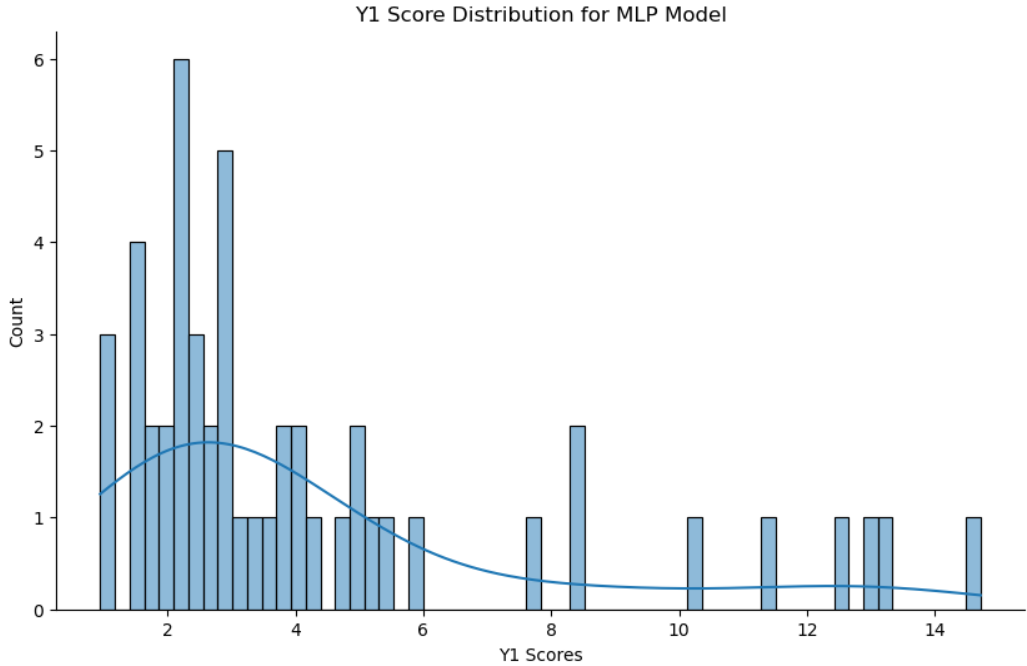
\includegraphics[width=1\textwidth]{./ReportImages/score_mlp_y1.png} 
    \caption{MLP Score statistics for 2D KPI(Mgrenz)} 
    \label{fig:MLP Score statistics for 2D KPI(Mgrenz)}
\end{figure}

\subsection{3D ETA Grid Results with \ac{MLP}}\label{sec:3D ETA Grid Results with MLP}

\begin{figure}[H]
    \centering
    \includegraphics[width=1\textwidth]{./ReportImages/KPI3Dprediction3.png} 
    \caption{1st MLP Training Results for 3D KPI(ETA)} 
    \label{fig:1st MLP Training Results for 3D KPI(ETA)}
\end{figure}

\begin{figure}[H]
    \centering
    \includegraphics[width=1\textwidth]{./ReportImages/KPI3Dprediction4.png} 
    \caption{2nd MLP Training Results for 3D KPI(ETA)} 
    \label{fig:2nd MLP Training Results for 3D KPI(ETA)}
\end{figure}

Since we are predicting a padded matrix to ensure dimensionality sync different ETA grids, the grid contains values even outside the boundard of the ETA envelope.
Hence, we attempted to slice the shape of the Torque curve from the ETA grid by by counting the number of columns a row to have based on consecutive values in the curve.
As you can see below, this has resulted in clipping some of the actual ETA envelope with the \ac{EM}'s operating drive cycle.\\
This brings us back to the point that it is imperative the prediction of the Torque curve is as good as possible to the actual curve as the envelope of the ETA grid is inherently dependent on it.


\begin{figure}[H]
    \centering
    \includegraphics[width=1\textwidth]{./ReportImages/KPI3Dprediction1.png} 
    \caption{3rd MLP Training Results for 3D KPI(ETA)} 
    \label{fig:3rd MLP Training Results for 3D KPI(ETA)}
\end{figure}

\begin{figure}[H]
    \centering
    \includegraphics[width=1\textwidth]{./ReportImages/KPI3Dprediction2.png} 
    \caption{4th MLP Training Results for 3D KPI(ETA)} 
    \label{fig:4th MLP Training Results for 3D KPI(ETA)}
\end{figure}


Observations from the predictions helped to correct few discrepancies in our development for instance in the ETA grid we replaced 0 with NAN values which we later understood were both represented different in the grid.\\
As efficiency values can take up values only between 0 and 100, we consider the same as constant across plots and use it as a baseline for determining the levels in the contour plot. \\ 
We have also left the output predictions for the Torque curve to remain as float values even when the target values are integers to preserve data precision. We give the client the flexibility to turn this on/off demand. \\
We also have the score statistics of how the model performs over the test dataset.\\

\begin{figure}[H]
    \centering
    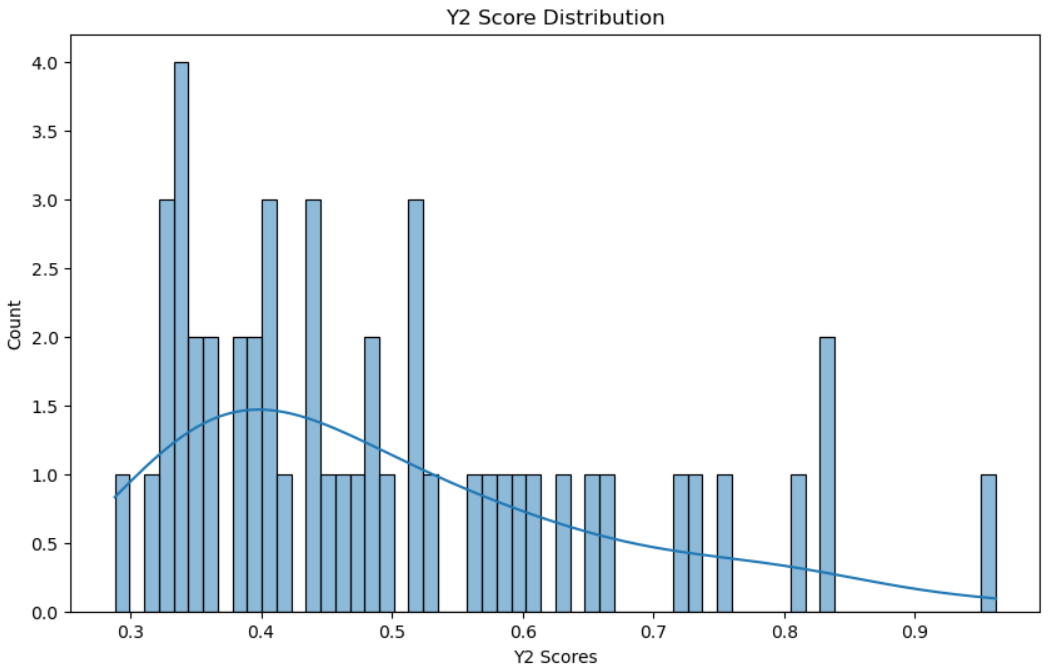
\includegraphics[width=1\textwidth]{./ReportImages/score_mlp_y2.png} 
    \caption{MLP Score statistics for 3D KPI(ETA)} 
    \label{fig:MLP Score statistics for 3D KPI(ETA)}
\end{figure}


We have used python 3.12.2 for our development and the pytorch library compatible with cuda.
The model was trained on a NVIDIA V100 GPU with blah blah.\\


\section{Results with Baseline}\label{sec:Results with Baseline}

From our observations of how the predictions closely resembled that of the target values, we have proceeded with a baseline model which is essentially the average of the target in all ground truth.
Based on the standard deviation of the target values with the baseline as is formulated in Equation CITE, the corresponding plots are generated.

%  Evaluation metric Y1 Element wise RMSE Loss for 2D KPI
\begin{equation}
    \text{Y1 Element wise RMSE} = \sqrt{\frac{1}{n} (\bar{x} - x_{i})^2} \quad \forall i \in \{0, \dots, w-1\}
    \label{eq:Y1 Element wise RMSE}
\end{equation}
    
    \textit{where
            \begin{itemize}
                \item n : \ac{EM} samples
                \item w : 1st dimension of 3D vector
                \item $\bar{x}$  : Baseline Average mean
            \end{itemize}
    }

The results of the Baseline model from inference is as below: \\

\subsection{2D Torque Curve Results with Baseline}\label{sec:2D Torque Curve Results with Baseline}

\begin{figure}[H]
    \centering
    \includegraphics[width=1\textwidth]{./ReportImages/KPI2D_predictions.png} 
    \caption{Baseline Results for 2D KPI(Mgrenz)} 
    \label{fig:MLP Training Results for 2D KPI(Mgrenz)}
\end{figure}

We also have the score statistics of how the Baseline model performs over the test dataset.\\

\begin{figure}[H]
    \centering
    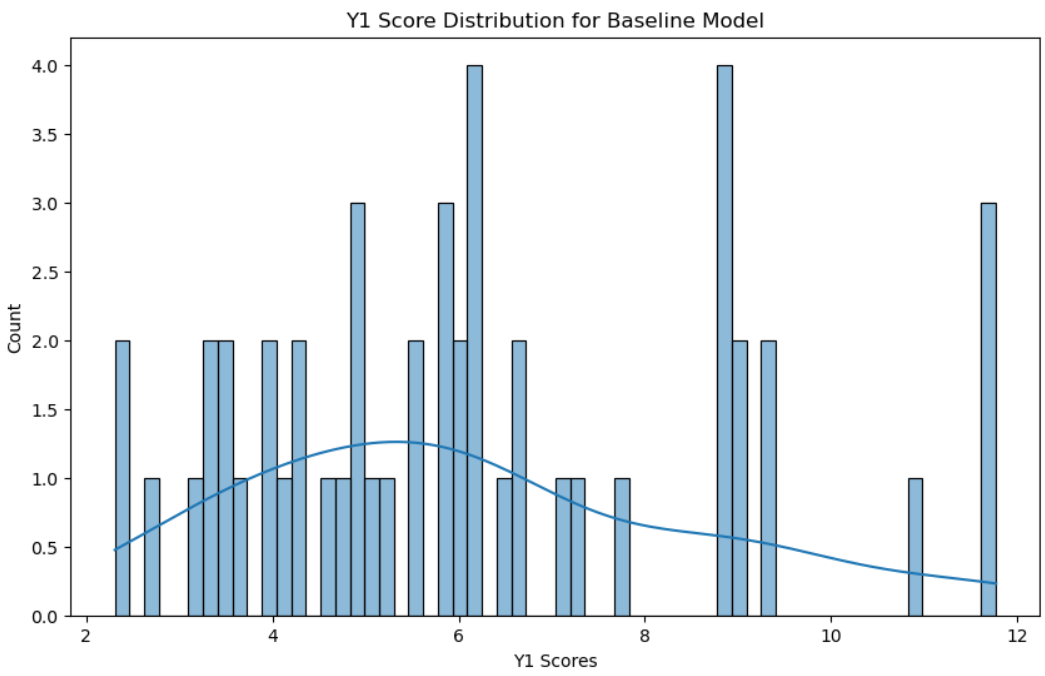
\includegraphics[width=1\textwidth]{./ReportImages/score_baseline_y1.png} 
    \caption{Baseline Score statistics for 2D KPI(Mgrenz)} 
    \label{fig:Baseline Score statistics for 2D KPI(Mgrenz)}
\end{figure}

\subsection{3D ETA Grid Results with Baseline}\label{sec:3D ETA Grid Results with Baseline}

\begin{figure}[H]
    \centering
    \includegraphics[width=1\textwidth]{./ReportImages/KPI3Dprediction3.png} 
    \caption{1st Baseline Results for 3D KPI(ETA)} 
    \label{fig:1st MLP Training Results for 3D KPI(ETA)}
\end{figure}

\begin{figure}[H]
    \centering
    \includegraphics[width=1\textwidth]{./ReportImages/KPI3Dprediction4.png} 
    \caption{2nd Baseline Results for 3D KPI(ETA)} 
    \label{fig:2nd MLP Training Results for 3D KPI(ETA)}
\end{figure}

We also have the score statistics of how the Baseline model performs over the test dataset.\\

\begin{figure}[H]
    \centering
    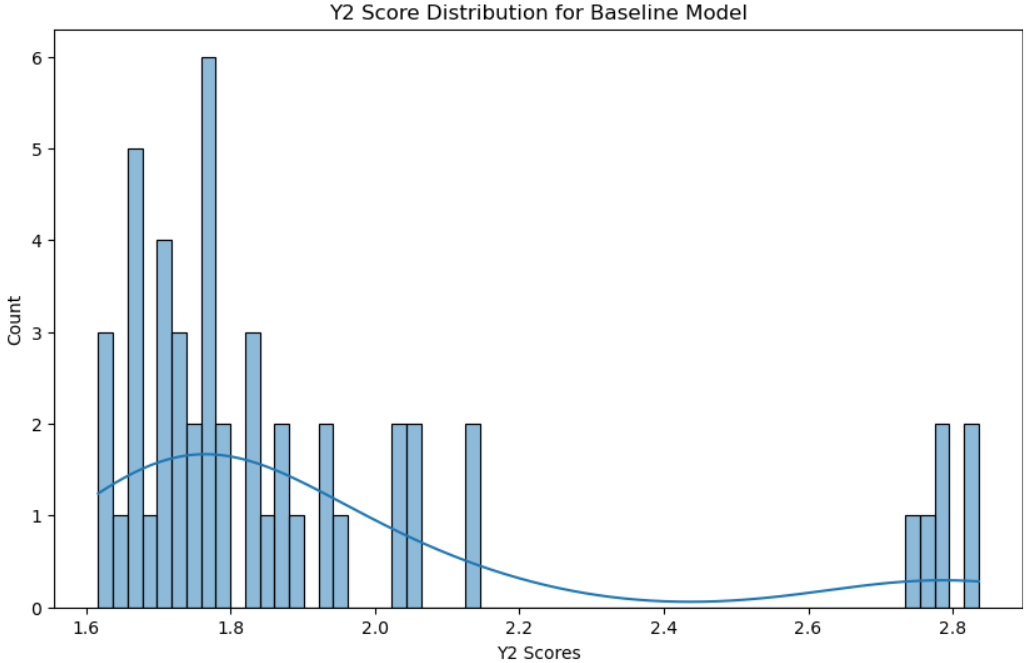
\includegraphics[width=1\textwidth]{./ReportImages/score_baseline_y2.png} 
    \caption{Baseline Score statistics for 3D KPI(ETA)} 
    \label{fig:Baseline Score statistics for 3D KPI(ETA)}
\end{figure}


\section{Ablation Studies}\label{sec:Ablation Studies}

As part of ablation studies, we have compared our evaluations of both the \ac{MLP} and the Baseline model on both targets respectively.

\begin{table}[H]
    \centering
    \begin{tabularx}{1\linewidth}{|X|X|X|}
    \hline {\bf Model} & {\bf Y1 Score} & {\bf Y2 Score}\\
    \hline 
    Baseline & 6.170 & 1.927 \\
    MLP & 5.1994 & 0.4962 \\
    \hline
    \end{tabularx}
    \caption{Ablation Studies}
    \label{tab:Ablation Studies}
\end{table}

We draw the inferences that our model has performed relatively better than the baseline for 2D KPI.
The inferences shown are strictly speaking from the Double V Magnet Topology which assumed the bulk of the data we had received.
\newpage 

\chapter{Conclusion}

This thesis offers a fresh outlook to the possibility of modelling the performance of an electric motor using \ac{GNN}s.
It also lays the foundation for future work on being able to generate electric motor design parameters conditioned on the 2 KPIs we predicted.

\section{Future Improvements}\label{sec:Future Improvements}

I would suggest the following improvements to our study : \cite{EHR HGNN-2024}
1. Build a model that uses the prediction from Y1 to predict its corresponding Y2. 
2. Although we have designed the model to be topology invariant for 3 topologies, we only had sufficient data from Double V Topology to draw evaluations from.
Further evaluations on the other topologies would be beneficial to critically assess our model's performance
3. Additionally, the motivation of building a topology invariant model was the reason we have considered building a heterogeneous graph to model the data. The machinery is elaborated in Section CIE.
Such a model could serve as yet another ablation study to our problem.
% India is described in \S\ref{part:Conclusion} 


\newpage 

\newpage 

\listoffigures

\newpage 

\newpage 

\listoftables

\newpage 

\newpage 

\begin{thebibliography}{00}

    \bibitem[01]{EHR HGNN-2024}
    \newblock Tsai Hor Chana, Guosheng Yina, Kyongtae Baeb, Lequan Yu 
    \newblock {\em Multi-task Heterogeneous Graph Learning on Electronic Health Records}.
    \newblock cs.LG, 14 Aug 2024.
    
    \bibitem[02]{SE HGNN-2023}
    \newblock Xiaocheng Yang, Mingyu Yan, Shirui Pan, Xiaochun Ye, Dongrui Fan
    \newblock {\em Simple and Efficient Heterogeneous Graph Neural Network}.
    \newblock cs.LG, 1 Sep 2023.

    \bibitem[03]{EV HGNN-2023}
    \newblock Xinru Huang
    \newblock {\em A Heterogeneous Graph Neural Network Model for Electric Vehicle Purchase Propensity Prediction}.
    \newblock ICDSCA, Oct 2023.
    
    \bibitem[04]{REF HGNN-2021}
    \newblock Qingsong Lv, Ming Ding, Qiang Liu, Yuxiang Chen, Wenzheng Feng, Siming He, Chang Zhou, Jianguo Jiang, Yuxiao Dong, Jie Tang
    \newblock {\em Are we really making much progress? Revisiting, benchmarking, and refining heterogeneous graph neural networks}.
    \newblock cs.LG, 30 Dec 2021.

    \bibitem[05]{ML HGNN-2023}
    \newblock Fredrik Johannessen; Martin Jullum
    \newblock {\em Finding Money Launderers Using Heterogeneous Graph Neural Networks}.
    \newblock ICDSCA, 25 July 2023.
    
    \bibitem[06]{PO GNN-2018}
    \newblock Damian Owerko, Fernando Gama, Alejandro Ribeiro
    \newblock {\em Predicting Power Outages Using Graph Neural Networks}.
    \newblock cs.LG, Nov 2018.

    \bibitem[07]{SM EMT-2020}
    \newblock Mikko Tahkola, Janne Keränen, Denis Sedov, Mehrnaz Farzam Far, Juha Kortelainen
    \newblock {\em Surrogate Modeling of Electrical Machine Torque Using Artificial Neural Networks}.
    \newblock ICDSCA, Dec 17 2020.
    
    \bibitem[08]{EM 2DFMP-2022}
    \newblock AKM Khaled Ahsan Talukder, Bingnan Wang and Yusuke Sakamoto
    \newblock {\em Electric Machine Two-dimensional Flux Map Prediction with Ensemble Learning}.
    \newblock ICEMS, 2022.

    \bibitem[09]{T-CNN-2024}
    \newblock Kazuhisa Iwata, Hidenori Sasaki, Hajime Igarashi, Daisuke Nakagawa, and Tomoya Ueda
    \newblock {\em Generalization Performance in Predicting Torque Characteristics Using Convolutional Neural Network and Stator Magnetic Flux.}
    \newblock ICDSCA, 3 Mar 2024.
    
    \bibitem[10]{EM MP-2021}
    \newblock Simone Ferrari, Paolo Ragazzo, Gaetano Dilevrano, Gianmario Pellegrino
    \newblock {\em Flux-Map Based FEA Evaluation of Synchronous Machine Efficiency Maps}.
    \newblock WEMDCD, 2021.

    \bibitem[11]{EM 2DFMP-2021}
    \newblock Vivek Parekh, Dominik Flore, Sebastian Schöps
    \newblock {\em Deep Learning-Based Prediction of Key Performance Indicators for Electrical Machines}.
    \newblock Jan 22, 2021.

    \bibitem[12]{EMAP-2020}
    \newblock Carlos Candelo-Zuluaga, Antonio Garcia Espinosa, Jordi-Roger Riba, Pere Tubert Blanch
    \newblock {\em Computationally Efficient Analysis of Spatial and Temporal Harmonics Content of the Magnetic Flux Distribution in a PMSM for Efficiency Maps Computation.}
    \newblock 2020.
    
    \bibitem[13]{EM SM-2023}
    \newblock Yihao Xu, Bingnan Wang, Yusuke Sakamoto, Tatsuya Yamamoto, and Yuki Nishimura
    \newblock {\em Comparison of Learning-based Surrogate Models for Electric Motors}.
    \newblock COMPUMAG, 2023.

    \bibitem[14]{IM HML-2021}
    \newblock Marius Stender, Oliver Wallscheid, Joachim Böcker
    \newblock {\em Accurate Torque Estimation for Induction Motors by Utilizing a Hybrid Machine Learning Approach}.
    \newblock PEMC, 2021.

    \bibitem[15]{EM FEM-2020}
    \newblock Katsuyuki Narita, Hiroyuki Sano, Nicolas Schneider, Kazuki Semba, Koji Tani, Takashi Yamada, Ryosuke Akaki
    \newblock {\em An Accuracy Study of Finite Element Analysis- based Efficiency Map for Traction Interior Permanent Magnet Machines}:
    \newblock 2020.
    
    \bibitem[16]{EM TL-2020}
    \newblock Jo Asanuma, Shuhei Doi, Hajime Igarashi
    \newblock {\em Transfer Learning Through Deep Learning: Application to Topology Optimization of Electric Motor}.
    \newblock 3 Mar 2020.

    \end{thebibliography}
\newpage 

\newpage 

\chapter*{Declaration on oath}
\addcontentsline{toc}{chapter}{Declaration on oath}

\vspace{1cm}

\noindent I hereby certify that I have written my master thesis independently and have not yet submitted it for examination purposes elsewhere. All sources and aids used are listed, literal and meaningful quotations have been marked as such.

\vspace{3cm}
\hfill\rule{15cm}{0.4pt} % Horizontal line for the signature aligned to the right

\begin{center}
    Lilly Abraham K64889, 11.12.2024 % Placeholder for the signature and date
\end{center}

\newpage 

\chapter*{Consent to Plagiarism Check}
\addcontentsline{toc}{chapter}{Consent to Plagiarism Check}
\vspace{1cm}

\noindent I hereby agree that my submitted work may be sent to PlagScan (www.plagscan.com) in digital form for the purpose of checking for plagiarism and that it may be temporarily (max. 5 years) stored in the database maintained by PlagScan as well as personal data which are part of this work may be stored there.

\vspace{0.5cm}

\noindent Consent is voluntary. Without this consent, the plagiarism check cannot be prevented by removing all personal data and protecting the copyright requirements. Consent to the storage and use of personal data may be revoked at any time by notifying the faculty.

\vspace{3cm}
\hfill\rule{15cm}{0.4pt} % Horizontal line for the signature aligned to the right

\begin{center}
    Lilly Abraham K64889, 11.12.2024 % Placeholder for the signature and date
\end{center}

\end{document}
